\chapter{Ingeniería de Riego por Gravedad}
\section{Descripción de los métodos y sistemas de riego por gravedad}
\subsection{Métodos y sistemas de riego por gravedad y sus variantes}
\begin{definition}[Método de riego]
    Se refiere a la forma o manera de hacer llegar el agua de riego a la zona de raíces de los cultivos
\end{definition}
\begin{definition}[Sistema de riego]
    Se refiere a los diversos componentes físicos que posibilitan la aplicación del agua de riego.
\end{definition}
Conviene aclarar que existen diversos nombre que se utilizan para referirse a los tipos y variantes de riego, que provienen de los diferentes criterios de clasificación que se han propuesto, todos ellos tratando de destacar ciertas características relevantes que los distinguen.
\begin{itemize}
    \item Riego superficial
    \item Por gravedad
    \item Aspersión
    \item Goteo
    \item Localizado en contraste con el riego extensivo
    \item Microirrigación
    \item Presurizado
    \item Riego de bajo volumen
    \item Subirrigación
    \item Subsuperficial
    \item Subterráneo
\end{itemize}
\subsection{Criterios de clasificación}
\begin{itemize}
    \item De acuerdo a la forma en que el agua se hace llegar a la zona de raíces de los cultivos:
    \begin{itemize}
        \item Superficiales, aéreos y subterráneos
    \end{itemize}
    \item De acuerdo al tipo de energía que utilizan para distribuir el agua en el área de cultivo \begin{itemize}
        \item Gravedad, presurizado
    \end{itemize}
    \item De acuerdo a la extensión de superficie de cultivo que humedecen \begin{itemize}
        \item Localizado y extensivo
    \end{itemize}
    \item De acuerdo a la magnitud del volumen de agua que utilizan \begin{itemize}
        \item Bajo volumen y gran volumen
    \end{itemize}
\end{itemize}
\begin{figure}[h!]
\centering
  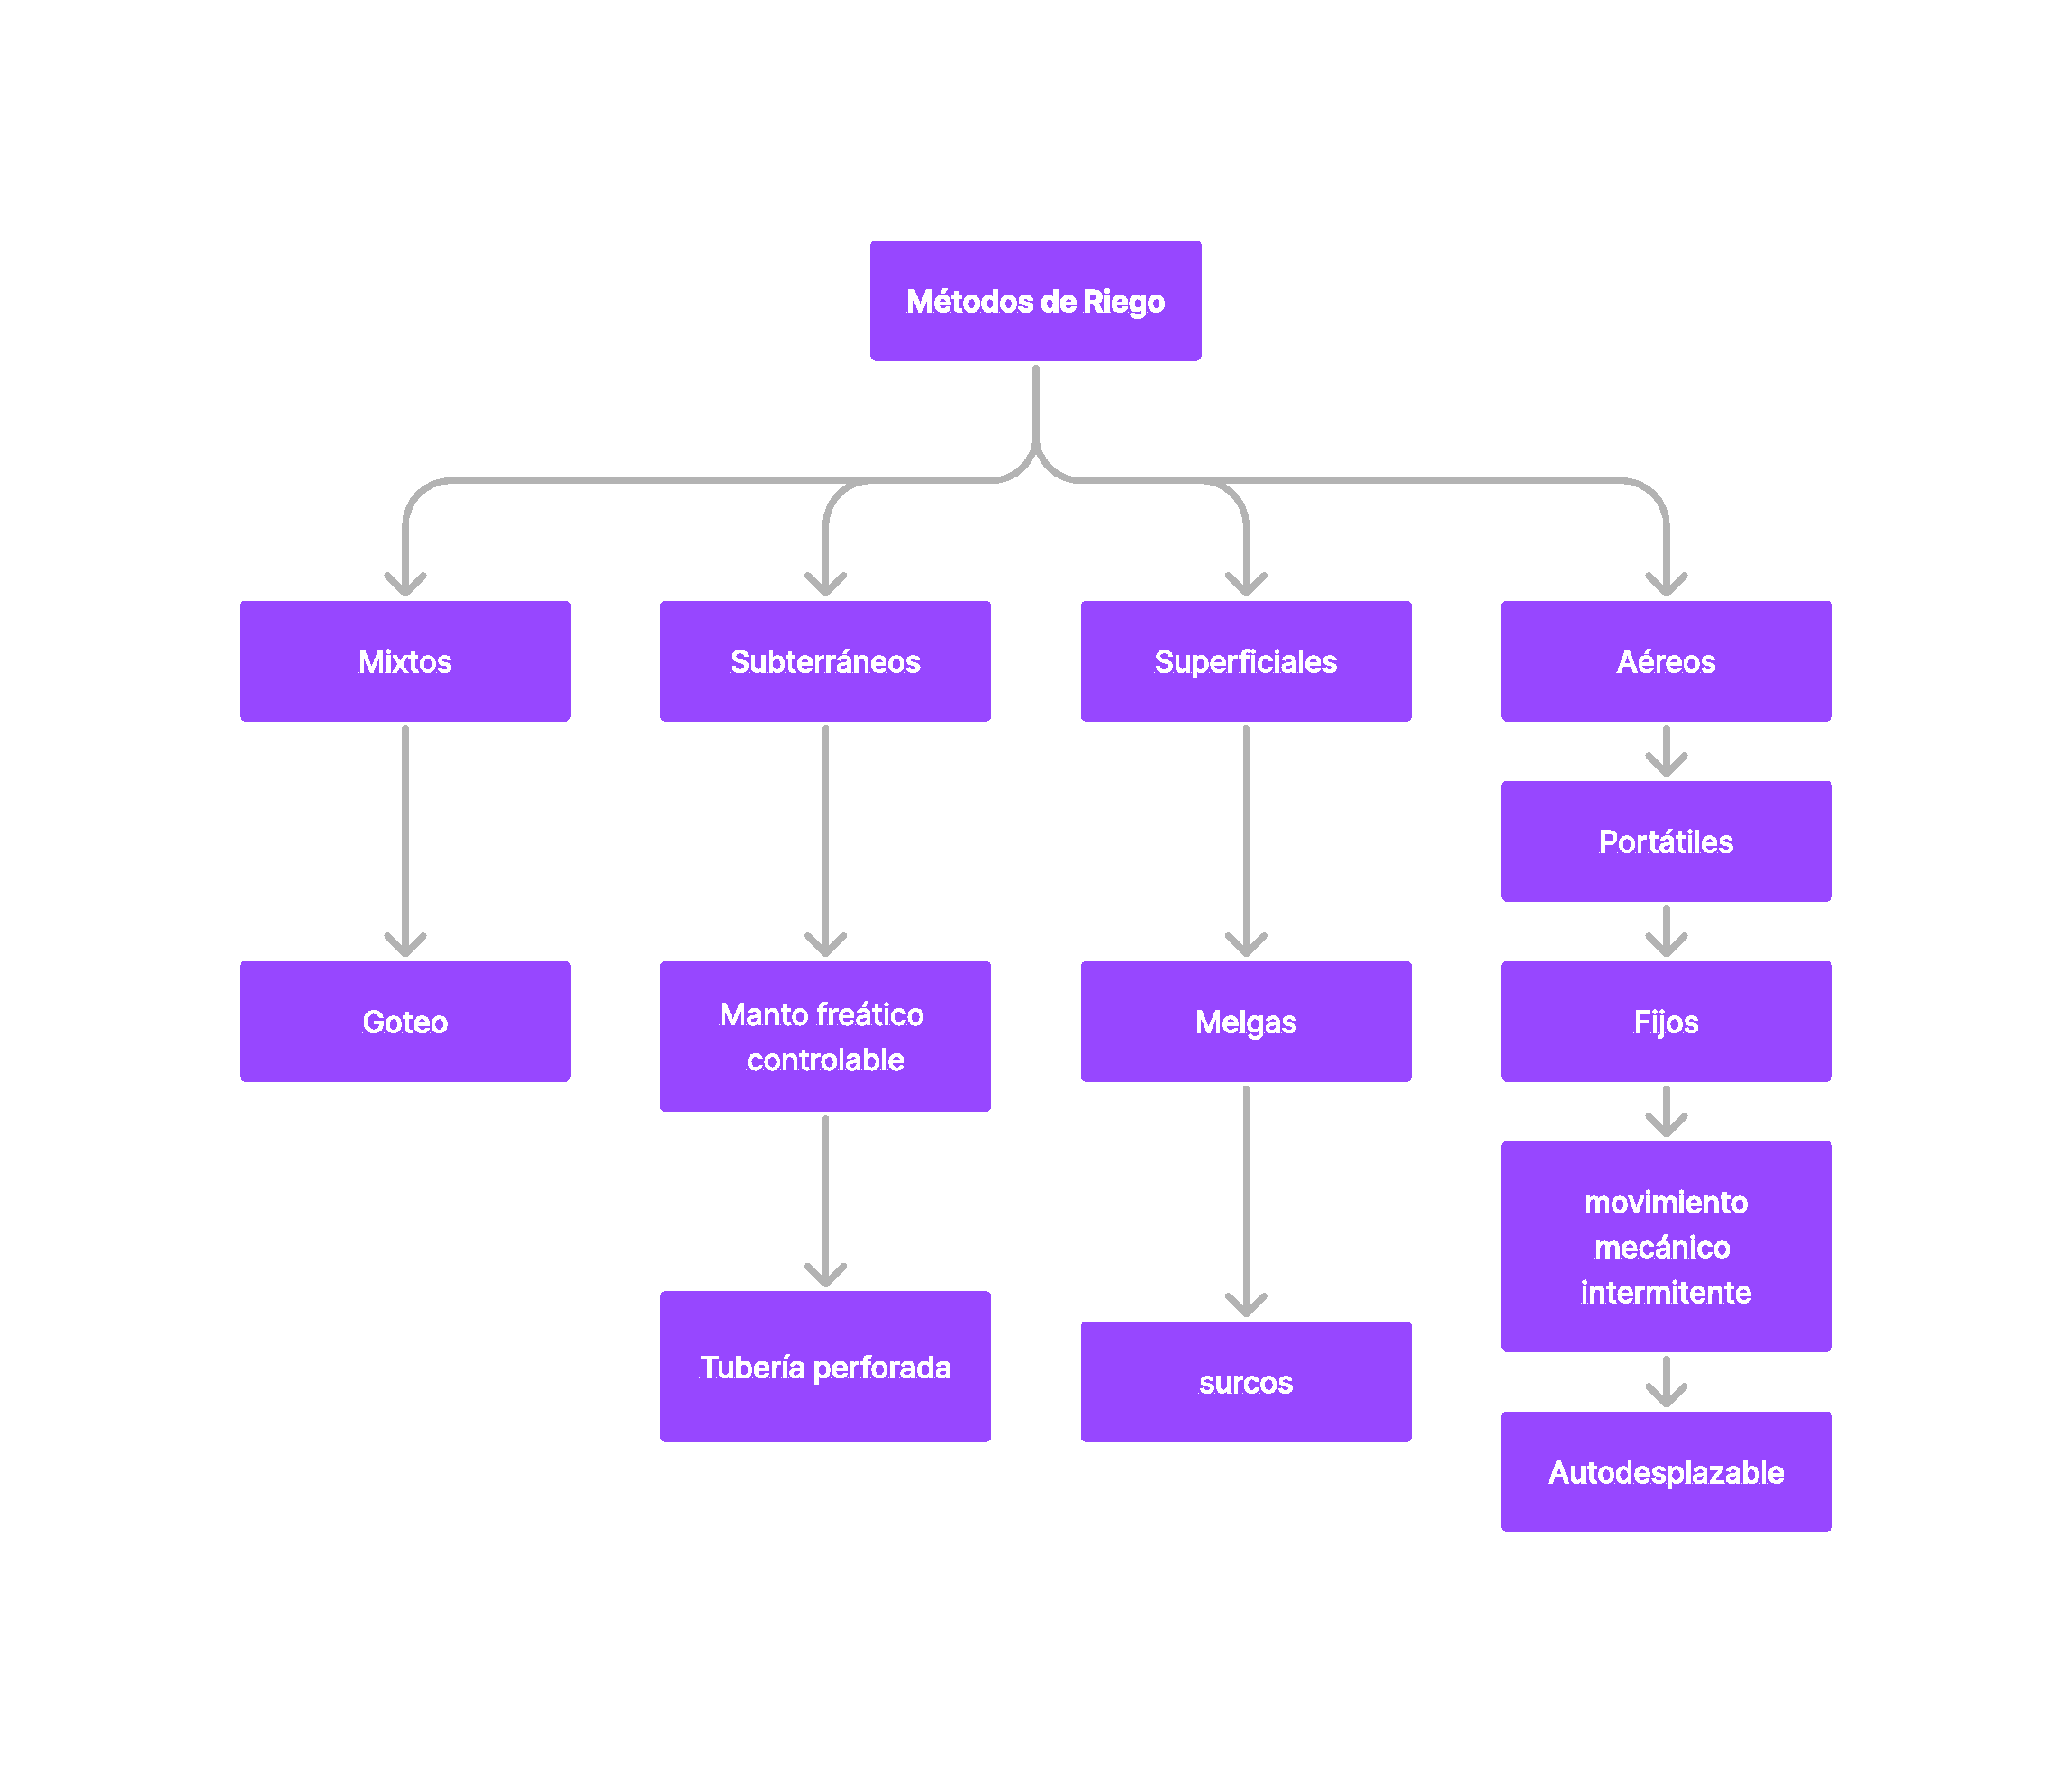
\includegraphics[width=1\textwidth]{r1.pdf}
  \caption{Sistema de clasificación de Israelsen}
  \label{r1}
\end{figure}
\Schema{-1.4ex}{15ex}
{\schemabox{Método\\ de\\ Riego}} { \Schema{-1ex}{8ex}
	{\schemabox{Gravedad}}
	{ \schema
		{\schemabox{Inundación total\\(melgas)}}
		{\schemabox{Rectas\\ A curva de nivel}}
		\medskip
		\schema
		{\schemabox{Inundación parcial\\ (surcos)}}
		{\schemabox{Rectos\\A curva de nivel}}
	}
	\Schema{-1ex}{5ex}
	{\schemabox{Presurizados}}
	{
		\vskip1ex\schemabox{Aspersión}
		\medskip
		\schemabox{Microaspersión}
		\medskip
		\schemabox{Goteo}
		\medskip
	}
}
\subsubsection{Riego por melgas}
Las melgas, son franjas de terreno generalmente de forma rectangular que se riegan en forma separada (independiente), delimitadas por bordos en el sentido longitudinal, que guían el flujo del agua hacia la parte inferior de la melga, y restringen el flujo lateral del agua. Aguas arriba se encuentran limitadas por la regadera o tubería de abastecimiento y aguas abajo pueden estar limitadas por un bordo transversal o por una zanja de desagüe (figura \ref{r2})
\begin{figure}[h!]
\centering
  \includegraphics[width=0.5\textwidth]{r2.jpg}
  \caption{Riego por melgas}
  \label{r2}
\end{figure}
Las melgas son especialmente usadas para cultivos de cobertura total como la alfalfa, pastos, trigo, cebada y avena, que no van a requerir labores de cultivo durante su ciclo (solamente el riego) y que soportan inundaciones por periodos mayores de 72 horas.

\subsubsection{Riego por surcos}
Los surcos son canales pequeños de diversas formas (secciones transversales), a lo que se introducen caudales de agua pequeños en la cabecera (extremo alto del surco). Así, el agua escurre por gravedad o por carga hidráulica, hacia el pie de la parcela (extremo bajo del surco), a medida que infiltra en el suelo a través de su perímetro mojado en forma radial (vertical y lateralmente), provocando solamente una inundación parcial de la superficie de cultivo.

El método de riego por surcos se adapta a muchos tipos de cultivos, principalmente a todos los que se siembran en hileras, como las gramíneas de porte alto, como el maíz, sorgo y la caña, o tales como el algodón, papa y todas las hortalizas.

Ventajas del riego por gravedad
\begin{itemize}
    \item Permite aplicar cantidades de agua grandes en poco tiempo
    \item Es aplicable a casi todos los cultivos
    \item Permite alcanzar eficiencias de riego altas con un buen diseño y manejo
    \item No exige alta calidad del agua
    \item No es afectado por el viento
\end{itemize}
\subsection{Riego por aspersión}
En éste método de riego el agua es conducida a presión por una red de tuberías para ser descargada sobre el cultivo y suelo en forma semejante a la lluvia, pero por supuesto en forma controlada
\subsubsection{Tipos de sistemas de RxA}
\begin{itemize}
    \item Sistemas fijos
    \item Sistemas portátiles y semiportátiles de movimiento manual
    \item Sistemas de desplazamiento mecánico intermitente
    \item Sistemas de desplazamiento mecánico continuo
\end{itemize}
Los componentes de un sistema de riego por aspersión son:
\begin{itemize}
    \item Equipo motobomba
    \item Tuberías
    \item Aspersores
    \item Accesorios
\end{itemize}
\begin{figure}[h!]
\centering
  \includegraphics[width=0.5\textwidth]{r3.png}
  \caption{Esquema de funcionamiento de un sistema de riego por aspersión portátil}
  \label{r3}
\end{figure}
\subsection{Sistemas de riego localizado}
\begin{itemize}
    \item Consisten en la aplicación del agua al suelo, pero humedeciendo solamente una zona restringida de volumen radicular
    \item No se moja todo el suelo del área cultivada
    \item Permiten aplicar cantidades pequeñas de agua y con alta frecuencia
    \item El nivel de humedad que se mantiene en el suelo es muy cercano al óptimo
\end{itemize}
\subsubsection{Tipos de sistemas de riego localizado}
\begin{itemize}
    \item Los sistemas que aplican el agua con un caudal no superior a los 20 L/h, por punto de emisión o por metro lineal de manguera, se les denomina sistemas de goteo
    \item Los sistemas que aplican el agua con un caudal superior a los 20 L/h e inferior a los 200 L/h, por punto de emisión, se denominan sistemas de microaspersión o de difusores
\end{itemize}
Componentes:
\begin{itemize}
    \item Cabezal o centro de control
    \item Tuberías
    \item Emisores
    \item Subunidad de riego
    \item Unidad de riego
    \item Unidad operacional
\end{itemize}
Ventajas de los sistemas de riego presurizado
\begin{enumerate}
    \item Su capacidad de salvar los desniveles topográficos
    \item Su capacidad de entregar el agua con rapidez y directamente donde debe de infiltrarse.
    \item Eliminan pérdidas de agua por conducción
    \item Permiten un control total y sencillo en la cantidad y en la velocidad de aplicación
    \item La capacidad de aplicar láminas de riego pequeñas con alta frecuencia
    \item La rapidez con que puede establecerse un proyecto de riego
\end{enumerate}
La regla de oro en el proceso de selección del método de riego, consiste en aceptar que ningún método o sistema es mejor que otro, ya que cada uno se adapta a condiciones diferentes y, manejados técnicamente pueden producir buenos resultados.
\subsubsection{Selección del riego por gravedad}
\begin{itemize}
    \item Los suelos son de textura media a fina, profundos, con alta capacidad de almacenamiento de agua
    \item Los terrenos son relativamente planos y uniformes o permiten una nivelación de precisión en forma económica
    \item El caudal de agua es relativamente grande pero disponible en periodos cortos de tiempo
    \item El costo del agua y de la tierra es bajo
    \item El nivel freático es profundo
    \item La mano de obra es abundante y barata
    \item Hay poca disponibilidad de capital inicial.
\end{itemize}
\subsubsection{Selección del riego por aspersión}
\begin{itemize}
    \item Los suelos son muy permeables o variables
    \item Los suelos son poco profundos para permitir una nivelación de precisión
    \item El relieve es muy accidentado por lo que los costos de nivelación son excesivos
    \item El suelo se erosiona fácilmente
    \item El caudal de agua es pequeño, pero disponible en cualquier momento que se requiera
    \item La mano de obra es escasa y cara
    \item En la zona no existen vientos fuertes por periodos prolongados de tiempo
    \item El agua no contiene altas concentraciones de sales
\end{itemize}
Los Sistemas de Riego por Goteo:
\begin{itemize}
    \item Requieren en general mayor inversión inicial
    \item Tienen mayores eficiencias de riego potenciales
    \item Son escasa o nulamente afectados por el viento
    \item Permiten utilizar aguas con altas concentraciones de sales
    \item Por sus características de alta uniformidad cuando son bien diseñados y operados, permiten aplicar los nutrientes en el agua de riego (fertirrigación), lo que aunado a la aplicación de riegos ligeros y frecuentes conducen a altos rendimientos y calidad de la producción
\end{itemize}
Los Sistemas de Riego por Aspersión:
\begin{itemize}
    \item Son especialmente útiles en la actualidad para cultivos forrajeros
    \item Requieren en general menor inversión inicial
    \item Son especialmente útiles para el establecimiento (germinación) de semillas pequeñas
    \item En determinadas circunstancia pueden emplearse para refrescar el ambiente y para el combate de heladas en algunos cultivos.
\end{itemize}

\subsection{Procesos y fases del riego por gravedad}
\subsubsection{Riego superficial}
\begin{enumerate}
    \item Avance
    \item Almacenamiento
    \item Consumo
    \item Recesión
\end{enumerate}

\subsubsection{Fase de avance}
\begin{figure}[h!]
	\centering
	\begin{subfigure}[b]{0.4\linewidth}
		\includegraphics[width=\linewidth]{r4.pdf}
		\caption{Inicia cuando se introduce el caudal en la cabecera de la melga o surco}
		\label{r4}
	\end{subfigure}
    \begin{subfigure}[b]{0.4\linewidth}
		\includegraphics[width=\linewidth]{r5.pdf}
		\caption{Esquema típico}
		\label{rg5}
	\end{subfigure}
	\begin{subfigure}[b]{0.4\linewidth}
		\includegraphics[width=\linewidth]{r6.pdf}
		\caption{Termina cuando el frente de humedecimiento llega al pie de la melga o surco}
		\label{rg6}
	\end{subfigure}
	\caption{Fase de avance}
	\label{rg4-6}
\end{figure}
\begin{table}[h!]
    \centering
    \begin{tabular}{@{}cc@{}}
    \toprule
    \begin{tabular}[c]{@{}c@{}}x\\ en metros\end{tabular} & \begin{tabular}[c]{@{}c@{}}tiempo\\ en minutos\end{tabular} \\ \midrule
    0   & 0   \\
    20  & 5   \\
    40  & 12  \\
    60  & 22  \\
    80  & 35  \\
    100 & 50  \\
    120 & 68  \\
    140 & 88  \\
    160 & 110 \\ \bottomrule
    \end{tabular}
    \caption{Pares de valores x, t del frente de avance (frente de humedecimiento), de la figura \ref{r5}}
    \label{tabr1}
\end{table}
Los factores que afectan al avance son:
\begin{itemize}
    \item Caudal
    \item Infiltración
    \item Pendiente
    \item Resistencia al flujo
\end{itemize}
\subsubsection{Fase de almacenamiento}
\begin{figure}[h!]
	\centering
	\begin{subfigure}[b]{0.4\linewidth}
		\includegraphics[width=\linewidth]{r7.pdf}
		\caption{Inicia cuando termina la fase de avance}
		\label{r7}
	\end{subfigure}
    \begin{subfigure}[b]{0.4\linewidth}
		\includegraphics[width=\linewidth]{r8.pdf}
		\caption{Esquema típico}
		\label{rg8}
	\end{subfigure}
	\begin{subfigure}[b]{0.4\linewidth}
		\includegraphics[width=\linewidth]{r9.pdf}
		\caption{Termina cuando se suspende el suministro de agua en la cabecera de la melga o surco}
		\label{rg9}
	\end{subfigure}
	\caption{Fase de almacenamiento}
	\label{rg7-9}
\end{figure}
Factores que afectan al almacenamiento
\begin{itemize}
    \item Caudal
    \item Tiempo de riego
    \item Infiltración
    \item Condición de frontera aguas abajo
\end{itemize}
\subsubsection{Fase de consumo (Retraso de la Recesión)}
\begin{figure}[h!]
	\centering
	\begin{subfigure}[b]{0.4\linewidth}
		\includegraphics[width=\linewidth]{r10.pdf}
		\caption{Inicia cuando se suspende el suministro de agua en la cabecera de la melga o surco.}
		\label{r10}
	\end{subfigure}
    \begin{subfigure}[b]{0.4\linewidth}
		\includegraphics[width=\linewidth]{r11.pdf}
		\caption{Termina cuando reaparece la superficie del terreno en algún punto de la melga o surco.}
		\label{rg11}
	\end{subfigure} 
	\caption{Fase de consumo}
	\label{rg10-11}
\end{figure}
Factores que afectan al consumo
\begin{itemize}
    \item Volumen almacenado en la superficie (condición inicial)
    \item Infiltración
    \item Pendiente
    \item Condición de frontera aguas abajo
\end{itemize}
\subsubsection{Fase de recesión}
\begin{figure}[h!]
	\centering
	\begin{subfigure}[b]{0.4\linewidth}
		\includegraphics[width=\linewidth]{r12.pdf}
		\caption{Inicia cuando reaparece la superficie del terreno en algún punto de la melga o surco.}
		\label{r12}
	\end{subfigure}
    \begin{subfigure}[b]{0.4\linewidth}
		\includegraphics[width=\linewidth]{r13.pdf}
		\caption{Esquema típico}
		\label{rg13}
	\end{subfigure}
	\begin{subfigure}[b]{0.4\linewidth}
		\includegraphics[width=\linewidth]{r14.pdf}
		\caption{Termina cuando toda la superficie del terreno queda descubierta de agua.}
		\label{rg14}
	\end{subfigure}
	\caption{Fase de recesión}
	\label{rg12-14}
\end{figure}
\begin{table}[h!]
    \centering
    \begin{tabular}{@{}cc@{}}
    \toprule
    \begin{tabular}[c]{@{}c@{}}x\\ en metros\end{tabular} & \begin{tabular}[c]{@{}c@{}}tiempo\\ en minutos\end{tabular} \\ \midrule
    0   & 120 \\
    20  & 11  \\
    40  & 125 \\
    60  & 128 \\
    80  & 131 \\
    100 & 135 \\
    120 & 139 \\
    140 & 144 \\
    160 & 150 \\ \bottomrule
    \end{tabular}
    \caption{Proceso: Pares de valores x, t de la cola de secado de la figura \textbackslash{}ref\{r13\}}
    \label{tabr2}
\end{table}
Factores que afectan a la recesión
\begin{itemize}
    \item Volumen almacenado en la superficie (C. I.)
    \item Infiltración
    \item Pendiente
    \item Condición de frontera aguas abajo
\end{itemize}
\begin{figure}[h!]
\centering
  \includegraphics[width=0.5\textwidth]{r15.pdf}
  \caption{Procesos y fases del riego superficial}
  \label{r15}
\end{figure}
\section{Nivelación de terrenos agrícolas}
\subsection{Importancia y beneficios de la Nivelación de terrenos agrícolas (NTA)}

Las condiciones de adaptabilidad para que el riego por gravedad funcione, principalmente es la nivelación del terreno, con la pendiente cercana a 0.

Necesidad Imperiosa: Uso Eficiente y Gestión Sustentable del Agua en la Agricultura

Opciones Viables:
\begin{itemize}
    \item Conversión de sistemas de riego por gravedad a sistemas de riego presurizado
    \item Mejoramiento del Riego por Gravedad \begin{itemize}
        \item Nivelación de Tierras
        \item Revestimiento de Canales
        \item Sustitución de canales por tubería
        \item Diseño y manejo apropiado del riego parcelario
    \end{itemize}
\end{itemize}

La nivelación de tierras, pretende solucionar los siguientes problemas de uso del agua en la agricultura del riego por gravedad:
\begin{itemize}
    \item Baja eficiencia de aplicación y
    \item Deficiente uniformidad del riego Ocasionados por las irregularidades topográficas
\end{itemize}
\subsubsection{Ventajas de la Nivelación de Tierras}
\begin{itemize}
    \item Ahorro de agua, mano de obra y energía
    \item Alta uniformidad en la aplicación del agua (con diseño y manejo adecuados)
    \item Mayor eficiencia en el uso de fertilizantes
    \item Operación más eficiente de la maquinaria
    \item Control de la erosión
    \item Mejoramiento del drenaje superficial
\end{itemize}
\subsubsection{Importancia de la Nivelación de Tierras}
La nivelación de tierras se justifica en cualquier proyecto de irrigación por gravedad, ya que generalmente se invierten sumas considerables en obras de captación y distribución, y comparativamente, se hacen inversiones bajas a nivel de la parcela, que es donde se refleja la bondad de todo un complejo sistema de irrigación

\subsubsection{Criterios de diseño de la nivelación de tierras agrícolas}
\begin{enumerate}
    \item Seleccionar la pendiente que maximice la efectividad de un sistema de riego existente o que se esté planeanado adoptar;
    \item Seleccionar la pendiente que minimice el movimiento de tierras.
\end{enumerate}
Una solución de compromiso entre ambos criterios parece lo más razonable

La nivelación de terrenos agrícolas, es una práctica de acondicionamiento físico del terreno, que consiste en la remoción de la tierra de las partes altas, su acarreo y depósito en las partes bajas, con el propósito de formar una superficie con pendiente uniforme, que se ajuste hasta donde sea posible a las pendientes naturales del terreno y que facilite las labores agrícolas, especialmente el riego.

\subsubsection{Planeación de los trabajos}
\begin{itemize}
    \item ¿Es adecuado su terreno para riego superficial?
    \item Seleccionar la época adecuada para realizar los trabajos
    \item Conocer los requerimientos de pendiente de la variante de riego superficial que se utilizará
\end{itemize}
\subsubsection{Casos en los que no es recomendable nivelar}
\begin{itemize}
    \item Suelos muy permeables
    \item Suelos someros
    \item Topografía ondulada
    \item Pendientes grandes
    \item Problemas de drenaje subsuperficial
    \item Suelos inestables
    \item Caudal disponible pequeño
\end{itemize}
\begin{table}[h!]
    \centering
    \begin{tabular}{@{}ccccccc@{}}
    \toprule
    \begin{tabular}[c]{@{}c@{}}Tipo de\\ riego\end{tabular} &
      \begin{tabular}[c]{@{}c@{}}Pendiente\\ mínima\end{tabular} &
      \multicolumn{4}{c}{Pendiente máxima} &
      \begin{tabular}[c]{@{}c@{}}Pendiente\\ ideal\end{tabular} \\ \midrule
    Melgas &
      0.05 &
      \begin{tabular}[c]{@{}c@{}}Zonas\\ áridas\\ 4\end{tabular} &
      \begin{tabular}[c]{@{}c@{}}Zonas\\ semiáridas\\ 3\end{tabular} &
      \begin{tabular}[c]{@{}c@{}}Zonas\\ semihúmedas\end{tabular} &
      \begin{tabular}[c]{@{}c@{}}Zonas\\ húmedas\end{tabular} &
      0.5 \\
    Surcos                                                    & 0.05 & 3 & 2 & 1 & 0.5                                                 & 0.4 \\
    \begin{tabular}[c]{@{}c@{}}Corruga-\\ ciones\end{tabular} & 1    & 6 & 4 & 2 & \begin{tabular}[c]{@{}c@{}}No\\ Recom.\end{tabular} & 2   \\ \bottomrule
    \end{tabular}
    \caption{Pendientes mínimas, máximas e ideales para diferentes variantes del riego por gravedad (\%)}
    \label{tabr3}
\end{table}
Las tecnologías para la nivelación son:
\begin{itemize}
    \item Tecnología tradicional
    \item Tecnología láser
    \item Tecnología GPS
\end{itemize}
\subsubsection{Tecnología tradicional}
\begin{itemize}
    \item Equipo topográfico tradicional
    \item Movimiento de tierras con maquinaria y equipo de control manual
\end{itemize}
Pasos para efectuar una nivelación tradicional
\begin{enumerate}
    \item Levantamiento topográfico
    \item Cálculo de las pendientes proyecto
    \item Cálculo de espesores de corte y relleno
    \item Estimación de volúmenes
    \item Ajuste a la elevación del plano proyecto
    \item Marcado del proyecto en el campo
    \item Ejecución y control de los trabajos
    \item Recepción de los trabajos y alisado final
\end{enumerate}
\subsubsection{Tecnología láser}
\begin{itemize}
    \item Equipo topográfico tradicional y/o equipo láser
    \item Movimiento de tierras con maquinaria y equipo de control automático con rayo láser
\end{itemize}
Pasos para nivelar con equipo láser
\begin{enumerate}
    \item Levantamiento topográfico
    \item Cálculo de las pendientes proyecto
    \item Movimiento de tierras
\end{enumerate}
Ventajas de la nivelación con equipo láser vs nivelación tradicional:
\begin{itemize}
    \item Levantamiento topográfico en menor tiempo, con menos personal y con menos posibilidades de cometer equivocaciones
    \item No requiere un estacado en cuadrícula
    \item No requiere emplear un sistema tedioso y tardado de control de los cortes y rellenos
    \item El movimiento grueso de tierras y el afine, se hace con una gran eficiencia y precisión
\end{itemize}
\subsection{Proyecto de la Nivelación de Terrenos Agrícolas}
\Schema{-1.4ex}{15ex}
{\schemabox{Métodos\\Empíricos}} { \Schema{-1ex}{4ex}
	{\schemabox{Perfil simple}}
	{  
		{\schemabox{Marr, 1957}}
		\medskip
		 
		{\schemabox{USDA, 1959}} 
	}
	\Schema{-1ex}{4ex}
	{\schemabox{Doble Perfil}}
	{
		\schemabox{Marr, 1957}
		\medskip
		\schemabox{USDA, 1959} 
	}
	\Schema{-1ex}{3ex}
	{\schemabox{Rectificación de\\curvas de nivel}}
	{
		\schemabox{(USDA 1961)}
	}
}

Como características, se tienen:
\begin{itemize}
  \item Métodos gráficos
  \item Soluciones subjetivas
  \item Varias propuestas antes de encontrar una solución aceptable
\end{itemize}

\Schema{-1.4ex}{15ex}
{\schemabox{Métodos\\Directos}} { \Schema{-1ex}{9ex}
	{\schemabox{Mínimos Cuadrados}}
	{ 
 % \schema
		{\schemabox{Marr, 1957}}
		\medskip
		% \schema
		{\schemabox{USDA, 1959}} 
  {\schemabox{Glvan, 1940}}
		\medskip
  {\schemabox{Chug, 1947}}
		\medskip
  {\schemabox{Marr, 1957}}
		\medskip
	  {\schemabox{Trueba, 1971}}
}
	\Schema{0ex}{2ex}
	{\schemabox{Centro de Volumen\\Fijo}}
	{
		\schemabox{Raju, 1960} 
	}
	\Schema{0ex}{2ex}
	{\schemabox{Residuos simétricos}}
	{
		\schemabox{(Shih y Kriz, 1971)}
	}
}
Como características, se tienen:
\begin{itemize}
  \item Métodos analíticos
  \item Solución única
  \item Solución óptima
\end{itemize}
En la actualidad, dependiendo de los recursos de cómputo disponibles, se puede elegir entre tres variantes del método de mínimos cuadrados 
\begin{enumerate}
  \item \textbf{MÉTODO GENERAL DE MÍNIMOS CUADRADOS} (Regresión Lineal Múltiple con dos variables independientes)
  
  REQUIERE: Calculadora de bolsillo programable o con Módulo deAplicación Estadístico con Regresión Lineal Múltiple.
  \item \textbf{MÉTODO DE MÍNIMOS CUADRADOS APLICADO A LOS PERFILES MEDIO} (Regresión Lineal Simple)

  REQUIERE: Calculadora de bolsillo (no necesariamente programable), que sea capaz de dar los parámetros de Regresión Lineal Simple.

  \item \textbf{MÉTODO DE LOS COEFICIENTES DE TRUEBA} (Versión original del Ing. Samuel Trueba Coronel)
  
  REQUIERE:
  \begin{enumerate}
    \item Calculadora de bolsillo con sólo las cuatro operaciones elementales (o incluso a mano).
    \item Listado de los llamados Coeficientes de Trueba
  \end{enumerate}
\end{enumerate}
Ecuación del plano proyecto
\begin{equation}
  \hat{Z}_{ij} = A + BX_i + CY_j
\end{equation}
\begin{notation}
  \begin{itemize}
    \item $\hat{Z}_{ij}=$ Cota sobre el plano proyecto en un punto de coordenadas $X_i,Y_j$
    \item $B,C=$ Pendientes en los sentidos de los ejes $X,Y$, respectivamente igual a constantes
    \item $A=$ Constante que geométricamente representa la cota sobre el plano proyecto en el origen del sistema de coordenadas
    \item $i=$ Número de hileras
    \item $j=$ Número de columnas
  \end{itemize}
\end{notation}
\begin{figure}[h!]
\centering
  \includegraphics[width=0.5\textwidth]{r16.pdf}
  \caption{Plano en el espacio tridimensional}
  \label{r16}
\end{figure}
\subsubsection{Principio de mínimos cuadrados}
El principio de Mínimos Cuadrados establece que:
\begin{theorem}
  Los mejores estimadores de los parámetros A,B,C se obtienen cuando la suma de cuadrados de las desviaciones (en este caso espesores de corte o relleno) se minimice
  \begin{equation}
    S = \sum_{ij} \left(Z_{ij} - \hat{Z}_{ij}\right)^2 = \sum_{ij} \left(Z_{ij} - A - BX_i - CY_j\right)^2 = \min 
  \end{equation}
  Utilizando la técnica del cálculo diferencial, para minimizar la expresión anterior, se obtiene sucesivamente:
  \begin{align}
    \frac{\partial S}{\partial A} = 0&& \frac{\partial S}{\partial B} = 0&& \frac{\partial S}{\partial C} = 0
  \end{align}
\end{theorem}
\subsubsection{Ecuaciones normales}
Combinando los resultados de las expresiones anteriores, se obtienen las llamadas ecuaciones normales:
\begin{align*}
  &NA       &&+ &&B \sum Z  &&+ &&C\sum Y   &&= &&\sum Z\\
  &A \sum X &&+ &&B\sum X^2 &&+ &&C\sum XY  &&= &&\sum XY\\
  &A\sum Y  &&+ &&B\sum XY  &&+ &&C\sum Y^2 &&= &&\sum YX
\end{align*}
Que en notación matricial quedan de la forma:
\begin{equation*}
  \begin{bmatrix}
      N&\sum X&\sum Y\\
      \sum X&\sum X^2&\sum XY\\
      \sum Y&\sum XY&\sum Y^2
  \end{bmatrix} \cdot \begin{bmatrix}
      &A\\
      &B\\
      &C
  \end{bmatrix} = \begin{bmatrix}
    &\sum Z\\
    &\sum XZ\\
    &\sum YZ
\end{bmatrix}
\end{equation*}
Por lo tanto:
\begin{equation}
  \begin{bmatrix}
    &A\\
    &B\\
    &C
\end{bmatrix} =
  \begin{bmatrix}
      N&\sum X&\sum Y\\
      \sum X&\sum X^2&\sum XY\\
      \sum Y&\sum XY&\sum Y^2
  \end{bmatrix}^{- 1} \cdot \begin{bmatrix}
    &\sum Z\\
    &\sum XZ\\
    &\sum YZ
\end{bmatrix}
\end{equation}
La solución por determinantes de las ecuaciones normales es como sigue:
\begin{align*}
  A = \frac{D_a}{D}&&B = \frac{D_b}{D}&& C = \frac{D_c}{D}
\end{align*}
Al mismo tiempo que, estas expresiones resultantes, son dobles sumatorias y N=nm= número total de vértices de la cuadrícula:
\begin{equation}
  \sum = \sum_{ij} =\sum_{i = 1}^{n}\cdot\sum_{j = 1}^{m}
\end{equation}
\subsubsection{Cortes y rellenos}
Los espesores de corte o relleno, en cada
punto de la cuadrícula, se calculan mediante:
\begin{equation}
  C_{ij} = Z_{ij} - \hat{Z}_{ij}
\end{equation}
\begin{notation}
  \begin{itemize}
    \item $C_{ij}=$ Espesores de corte (valores positivos) o espesores de relleno (valores negativos), en m;    
    \item $Z_{ij}=$ Cotas del terreno natural, en m;
    \item $\hat{Z}_{ij}=$ coordenadas de cada punto de la cuadrícula, en la ecuación del plano proyecto, en m.    
  \end{itemize}
\end{notation}
\subsubsection{Cubicación: Método de la adición}
Este método es el más sencillo, pero también el menos preciso. El volumen total de corte y relleno, se calculan mediante las ecuaciones indicadas. 
\begin{align*}
  V_c = L^2 \sum_{i = 1}^{Nc} C_i\\
  V_r = L^2 \sum_{j = 1}^{Nr} \left\lvert R_i \right\rvert \\
\end{align*}
\begin{notation}
  \begin{itemize}
    \item $V_c=$ Volumen total de corte, en $m^3$
    \item $C_i=$ Espesor de corte i-ésimo, en m
    \item $i= 1,2,3...N_c$: Número de espesor de corte
    \item $V_r=$ Volumen total de relleno, en $m^3$
    \item $R_j=$ Espesor de relleno j-ésimo, en m
    \item $j=1,2,3...R_c$: Número de espesor de relleno.
  \end{itemize}
\end{notation}
El volumen calculado es el volumen de todo el proyecto.
\subsubsection{Cubicación: Método de los cuatro vértices}
Un método más preciso, recomendado por el SCS del USDA, es el llamado método de los cuatro vértices. Sin embargo, el cálculo es más laborioso porque es aplicable a las áreas individuales, $L^2$, en cuyos vértices se conocen los datos de construcción. Los volúmenes de corte y relleno, se calculan mediante:
\begin{align}
  &\tilde{V}_c = \frac{L^2}{4}\cdot \frac{\left(\sum C\right)^2}{\sum C + \left\lvert \sum R\right\rvert }\\
  &\tilde{V}_r = \frac{L^2}{4}\cdot \frac{\left(\sum R\right)^2}{\sum C + \left\lvert \sum R\right\rvert }
\end{align}
\begin{notation}
  \begin{itemize}
    \item $\tilde{V}_c=$ Volumen de corte en el cuadrado correspondiente, en $m^3$
    \item $\tilde{V}_r=$ Volumen de relleno en el cuadrado correspondiente, en $m^3$
    \item $\sum C=$ Suma de espesores de corte en los vértices del cuadrado correspondiente
    \item $\sum R=$ Suma de espesores de relleno en los vértices del cuadrado correspondiente
  \end{itemize}
\end{notation}
Los volúmenes de corte y relleno calculados con este método, son volúmenes en cada uno de los cuadros de la cuadrícula
\subsubsection{Abundamiento y compactación durante el movimiento de tierra}
En un proyecto de nivelación de terrenos, el volumen de excavación resultante con el plano de mejor ajuste, que equilibra los datos de construcción, deberá aumentarse para tomar en cuenta el efecto de compactación que se produce el tránsito normal del equipo.

\subsection{Ajuste a la elevación del plano proyecto ($\Delta$)}
En un proyecto de nivelación de terrenos, el volumen de excavación resultante con el plano de mejor ajuste, que equilibra los datos de construcción, deberá aumentarse para tomar en cuenta el efecto de compactación que se produce el tránsito normal del equipo

Relación $V_c/V_r > 1.0$
\begin{equation}
  \Delta = \frac{Q\sum_{j = 1}^{N_r}\left\lvert R_j\right\rvert - \sum_{i = 1}^{N_c}C_i}{QN_r + N_c}
\end{equation}
Estimación de $\Delta$:
\begin{equation}
  \frac{V_c}{V_r} = \frac{L^2 \sum_{i = 1}^{N_c}C_i}{L^2 \sum_{j = 1}^{N_r}\left\lvert R_j\right\rvert} = Q > 1
\end{equation}
Despejando:
\begin{equation*}
  Q =\frac{L^2 \sum_{i = 1}^{N_c}C_i +L^2 N_c\Delta }{L^2 \sum_{j = 1}^{N_r}\left\lvert R_j\right\rvert - L^2 N_r\Delta}  \implies \Delta =\frac{Q\sum_{j = 1}^{N_r}\left\lvert R_j\right\rvert -\sum_{i = 1}^{N_c}C_i }{QN_r + N_c}
\end{equation*}
Coordenadas centroidales del terreno: ($X_c, Y_c, Z_c$)
\begin{equation}
  Z_c = \frac{\sum_{i,j}^{n,m} Z_{ij}}{n \cdot m}
\end{equation}
\subsubsection{Cubicación con el método de los cuatro vértices y método racional}
\begin{figure}[h!]
\centering
  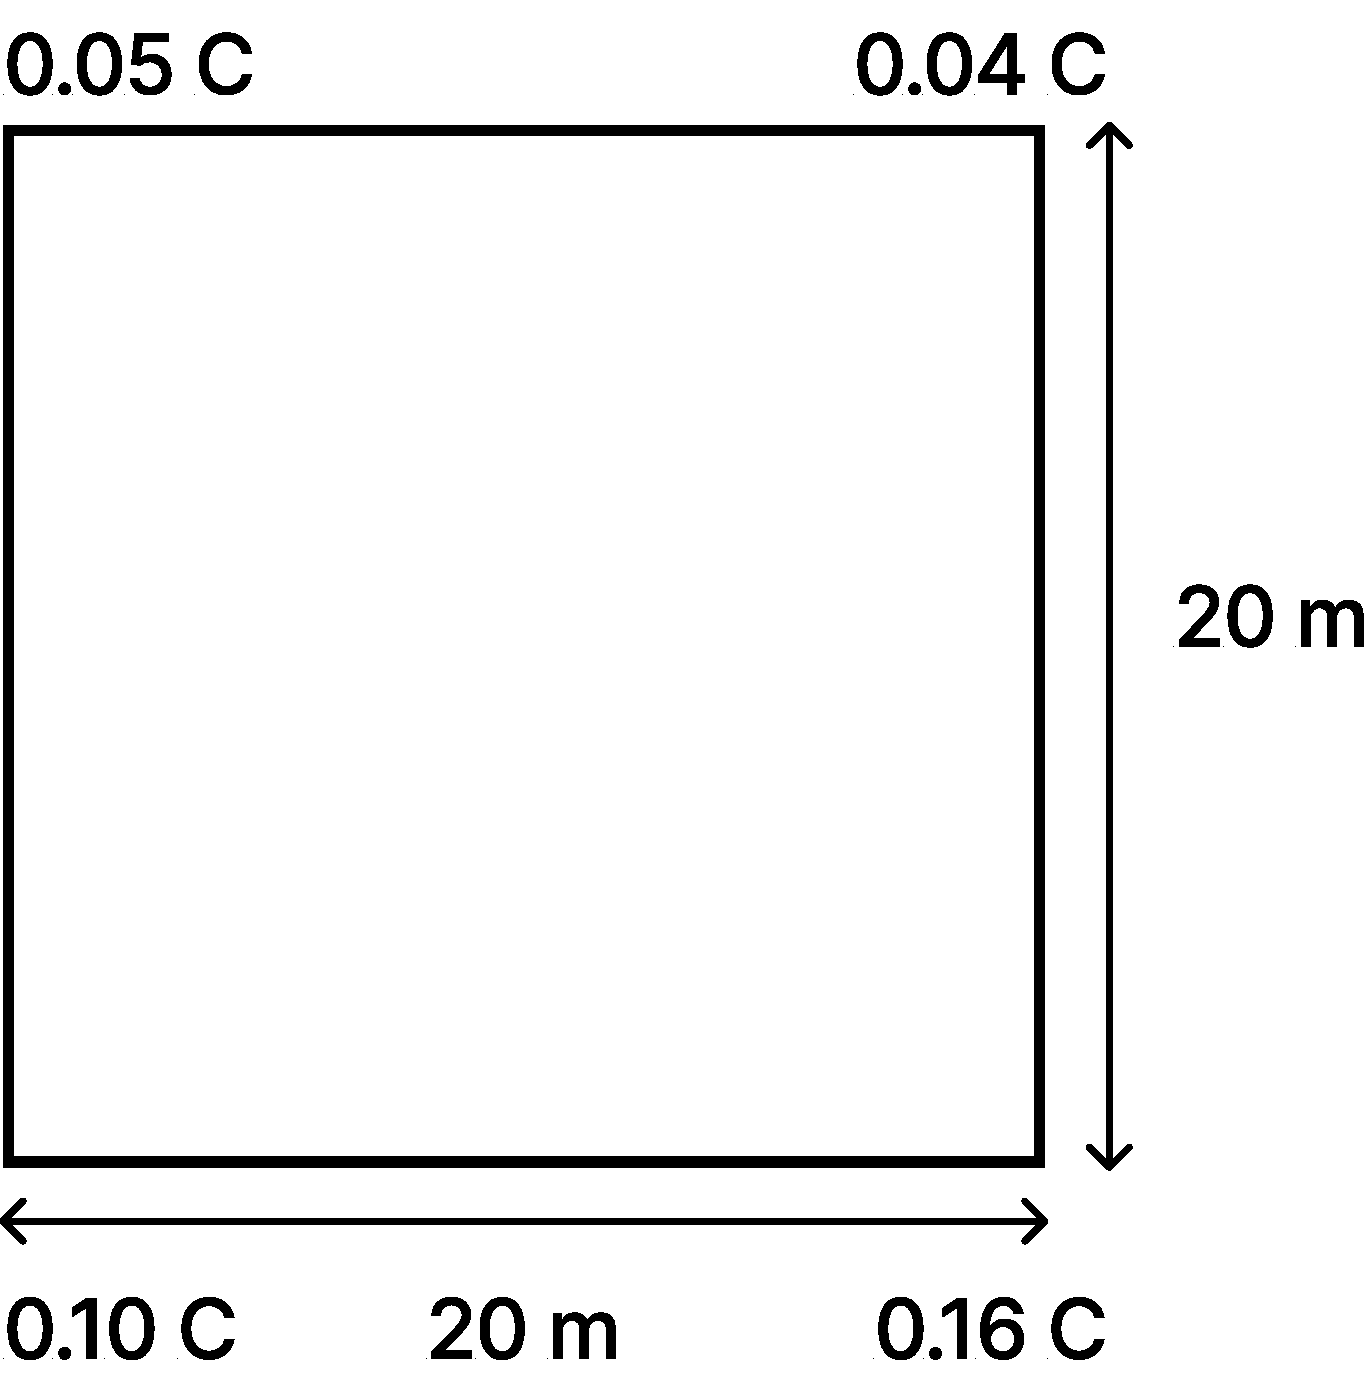
\includegraphics[width=0.5\textwidth]{r17.pdf}
  \caption{Esquema del problema, primer caso}
  \label{r17}
\end{figure}
En el primer caso (figura \ref{r17}), con el método de los cuatro vértices tenemos:
\begin{align*}
    &V_c =\frac{L^2}{4}\frac{\left(\sum C\right)^2}{\sum C + \sum\left\lvert R\right\rvert } = \frac{100(0.35)^2}{0.35} =35m^3\\
    &V_r = \frac{L^2}{4} \frac{\left(\sum R\right)^2}{\sum C + \sum\left\lvert R\right\rvert} =0m^3
\end{align*}
Con el método racional (promedio)
\begin{equation*}
    V_c =\frac{\frac{0.35}{4}}{400} =35m^3
\end{equation*}
\begin{figure}[h!]
\centering
  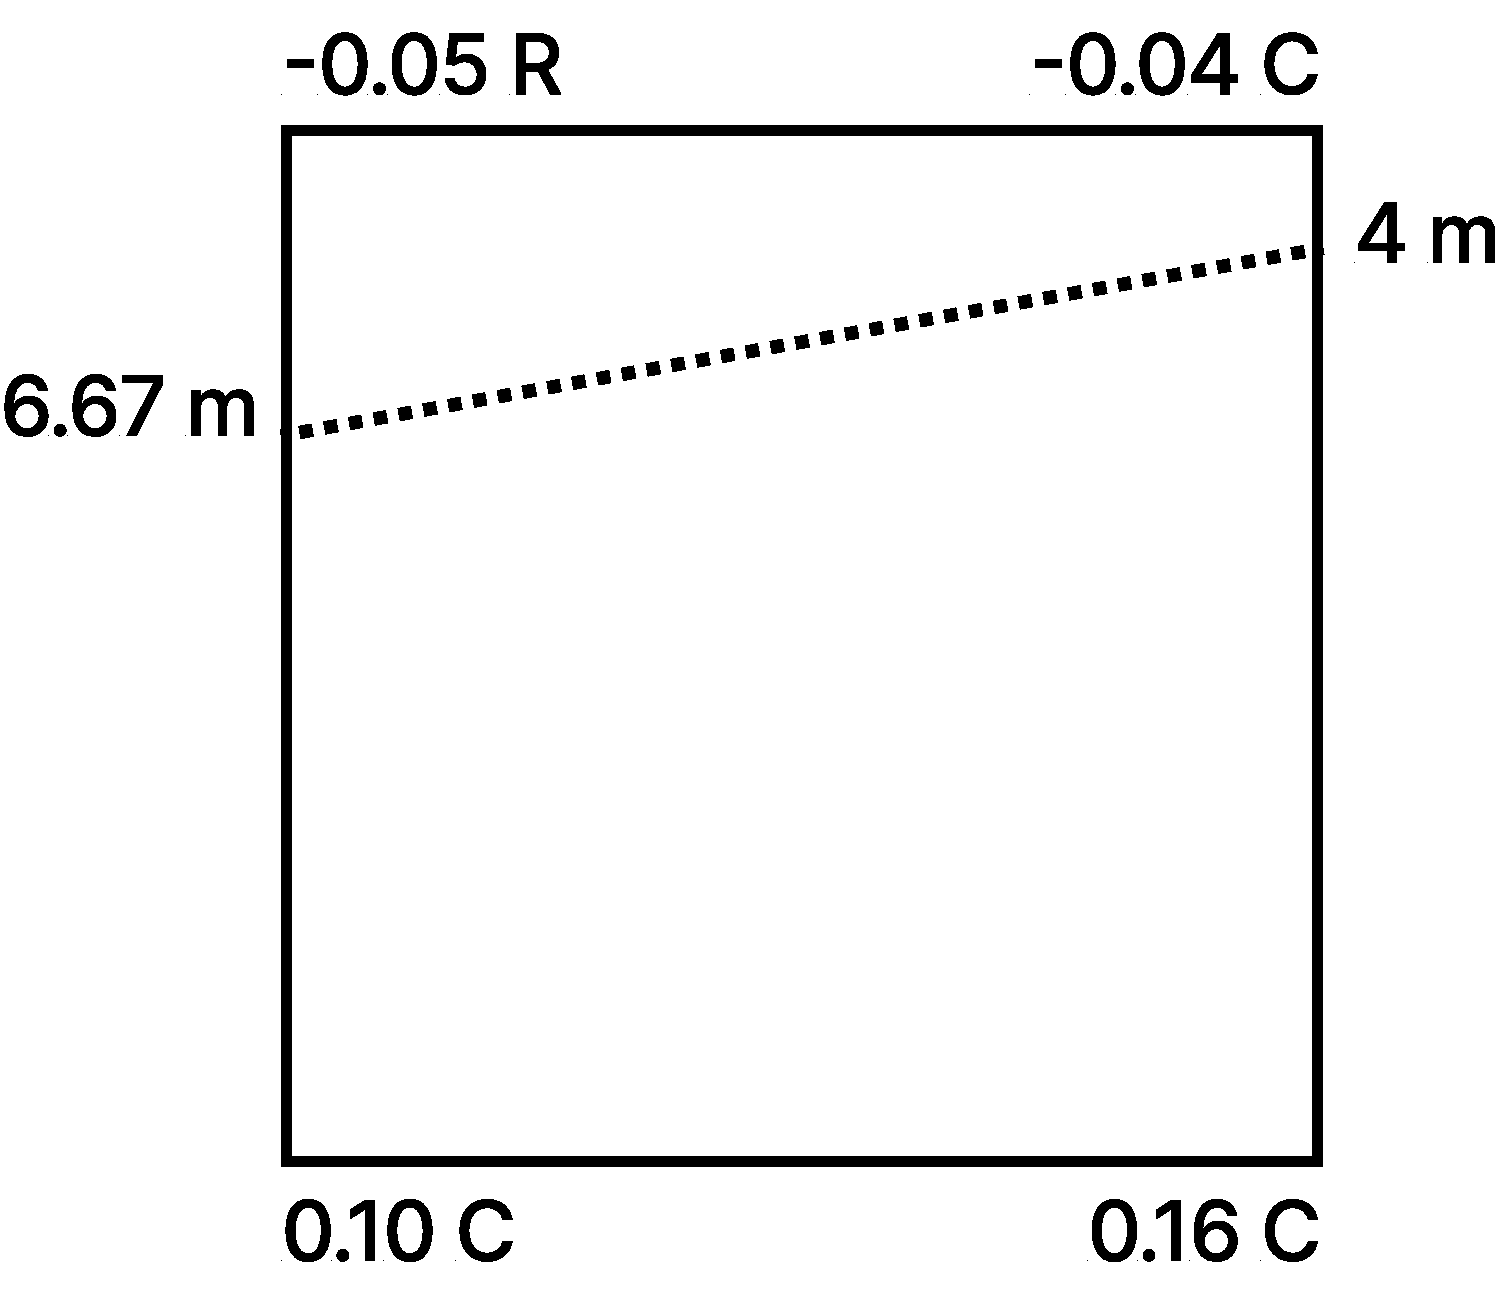
\includegraphics[width=0.5\textwidth]{r18.pdf}
  \caption{Segundo caso}
  \label{r18}
\end{figure}
En el segundo caso (figura \ref{r18}), con el método de los cuatro vértices:
\begin{align*}
    &V_c =\frac{L^2}{4}\frac{\left(\sum C\right)^2}{\sum C + \sum\left\lvert R\right\rvert } = \frac{100(0.26)^2}{0.35} =19.31^3\\
    &V_r = \frac{L^2}{4} \frac{\left(\sum R\right)^2}{\sum C + \sum\left\lvert R\right\rvert} = \frac{100(0.09)^2}{0.35} =2.31m^3
\end{align*}
Con el método racional (promedios)
\begin{align*}
        &\frac{0.05}{0.15} \cdot 20 = 6.67m&&\frac{0.04}{0.20} \cdot 20 = 4m \\
        &A_r = \frac{6.67 + 4}{2}\cdot 20 = 106.7m^2&& A_c = 400 - 106.7 = 293.3m^2\\
        &V_c = \left(\frac{0.26}{4}\right)\left(293.3\right) = 19.06m^3&& V_r = \left(\frac{0.09}{4}\right)\left(106.70\right) =2.4m^3
\end{align*}
\begin{figure}[h!]
\centering
  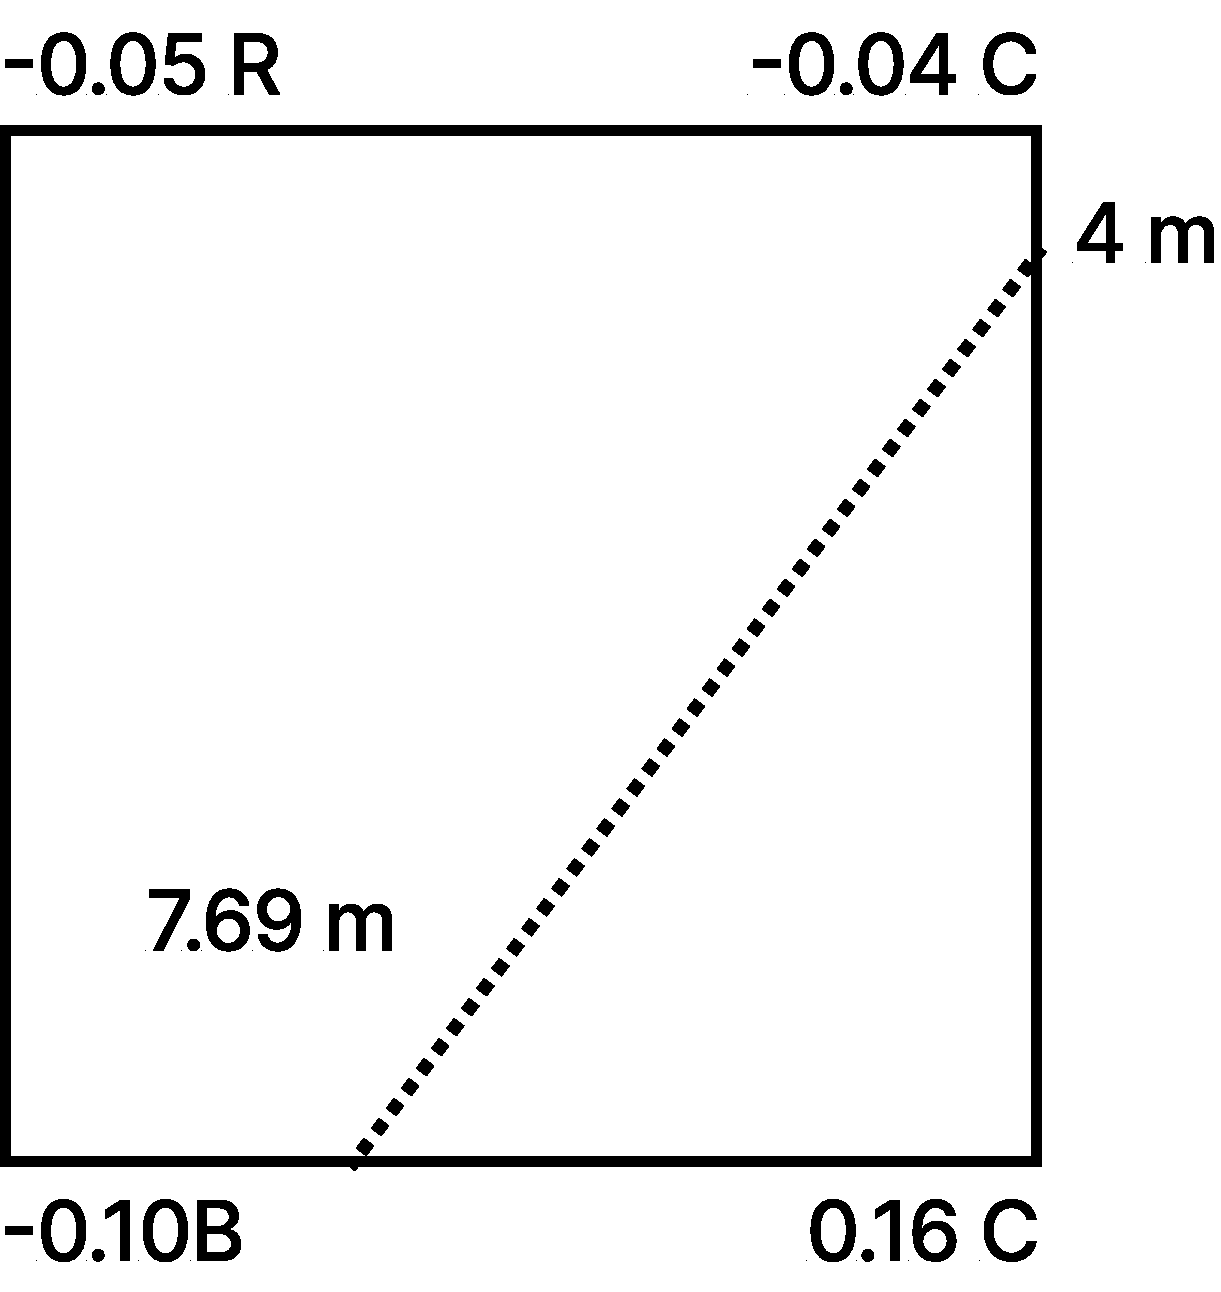
\includegraphics[width=0.5\textwidth]{r19.pdf}
  \caption{Caso 3}
  \label{r19}
\end{figure}
Por último en el caso tres de la figura \ref{r19}, obtenemos con el método de los cuatro vértices:
\begin{align*}
    &V_c ==\frac{L^2}{4}\frac{\left(\sum C\right)^2}{\sum C + \sum\left\lvert R\right\rvert } = \frac{100(0.16)^2}{0.35} =7.31m^3\\
    &V_r = \frac{L^2}{4} \frac{\left(\sum R\right)^2}{\sum C + \sum\left\lvert R\right\rvert} = \frac{100(0.19)^2}{0.35} =10.31m^3
\end{align*}
Y con el método racional (promedios)
\begin{align*}
    &\frac{0.10}{0.26} \cdot 20 = 7.69 m&&\frac{0.04}{0.20} \cdot 20 = 4m \\
    &A_C = \frac{(20 - 7.69)(16)}{2}\cdot 20 = 98.48 m^2&& A_r = 400 - 98.48 = 301.52 m^2\\
    &V_c = \left(\frac{0.16}{3}\right)\left(98.48\right) = 5.25 m^3&& V_r = \left(\frac{0.19}{5}\right)\left(301.52\right) = 11.46 m^3
\end{align*}

\subsection{Levantamiento topográfico para el proyecto de NTA}
\subsubsection{Método de Mínimos Cuadrados aplicado a los perfiles promedio}
Note que mediante los perfiles promedio, se transformó un problema del espacio tridimensional en dos problemas del espacio de bidimensional
\begin{figure}[h!]
\centering
  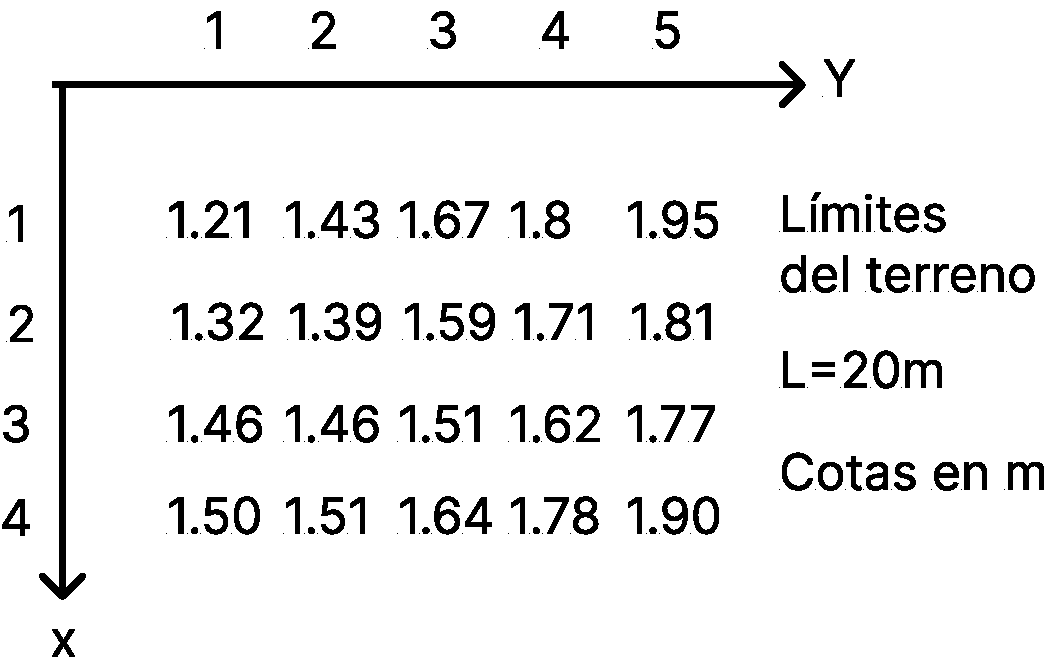
\includegraphics[width=0.5\textwidth]{r20.pdf}
  \caption{Datos de campo}
  \label{r20}
\end{figure}
\begin{table}[h!]
    \centering
    \begin{tabular}{@{}cccccccc@{}}
    \toprule
                            &        &        &        &        &                           & $\sum_{j=1}^{m} Z_{ij}$ & $\bar{Z}_i$ \\ \midrule
                            & 1.21   & 1.43   & 1.67   & 1.80   & \multicolumn{1}{c|}{1.95} & 8.06                    & 1.612       \\
                            & 1.32   & 1.39   & 1.59   & 1.71   & \multicolumn{1}{c|}{1.81} & 7.82                    & 1.564       \\
                            & 1.46   & 1.46   & 1.51   & 1.62   & \multicolumn{1}{c|}{1.77} & 7.82                    & 1.564       \\
                            & 1.5    & 1.51   & 1.64   & 1.78   & \multicolumn{1}{c|}{1.90} & 8.33                    & 1.666       \\
    $\sum_{i=1}^{n} Z_{ij}$ & 5.49   & 5.79   & 6.41   & 6.91   & \multicolumn{1}{c|}{7.43} & 32.03                   &             \\ \midrule
    $\bar{Z}_j$             & 1.3725 & 1.4475 & 1.6025 & 1.7275 & 1..8575                   &                         &             \\ \bottomrule
    \end{tabular}
    \caption{Cálculos}
    \label{tabr4}
\end{table}
\begin{table}[h!]
  \centering
  \begin{tabular}{@{}cccc@{}}
  \toprule
  \multicolumn{2}{c}{\begin{tabular}[c]{@{}c@{}}Perfil medio en \\ la dirección X\end{tabular}} &
    \multicolumn{2}{c}{\begin{tabular}[c]{@{}c@{}}Perfil medio en\\ la dirección Y\end{tabular}} \\ \midrule
  $X_i$                       & $\bar{Z}_i$                       & $Y_j$               & $\bar{Z}_j$              \\ \midrule
  20                          & 1.612                             & 20                  & 1.3725                   \\
  40                          & 1.564                             & 40                  & 1.4475                   \\
  60                          & 1.564                             & 60                  & 1.6025                   \\
  80                          & 1.666                             & 80                  & 1.7275                   \\ \cmidrule(r){1-2}
  \multicolumn{2}{c}{\multirow{2}{*}{$Z_i = 0.00081x + 1.56100$}} & 100                 & 1.8575                   \\ \cmidrule(l){3-4} 
  \multicolumn{2}{c}{}                                            & \multicolumn{2}{c}{$Z_i = 0.00625y + 1.22650$} \\ \bottomrule
  \end{tabular}
  \caption{Tabulación del Perfil medio en la dirección X,Y}
  \label{tabr5}
  \end{table}
Haciendo una regresión lineal simple:
\begin{align*}
    &\hat{Z}_i = a + BX_i\\
    &S =\sum_{i = 1}^n\left(Z_i - \hat{Z}_i \right)^2 = \min\\
    &S =\sum_{i = 1}^n\left(Z_i - a - BX_i \right)^2 = \min\\
    &\frac{\partial S}{\partial a} = 0;\quad \frac{\partial S}{\partial B} = 0\\
    & \frac{\partial S}{\partial a} = - 2\sum_{i = 1}^n \left(\bar{i} - a - BX_i \right) = 0\\
    &\frac{\partial S}{\partial B} = - 2\sum_{i = 1}^{n}\left(\bar{Z}_i - a - BX_i \right)X_i = 0\\
    & an + B \sum_{i = 1}^{n} X_i = \sum_{i = 1}^{n} \bar{Z}_i\\
    & \sum_{i = 1}^{n} X_i + B \sum_{i = 1}^{n} X_i^2 = \sum_{i = 1}^{n}X_i \bar{Z}_i\\
    & a = \frac{\sum_{i= 1}^{n}\bar{Z}_i - B\sum_{i = 1}^{n} X_i}{n}\\
    & \left(\frac{\sum_{i= 1}^{n}\bar{Z}_i - B\sum_{i = 1}^{n} X_i}{n}\right) \sum_{i= 1}^{n}X_i - B\sum_{i = 1}^{n} X_i^2 = \sum_{i= 1}^{n}\bar{Z}_i - B\sum_{i = 1}^{n} X_i \bar{Z}_i\\
    &\left(\sum_{i= 1}^{n}\bar{Z}_i - B\sum_{i = 1}^{n} X_i\right)\sum_{i= 1}^{n}X_i + nB\sum_{i = 1}^{n} X_i = n\sum_{i= 1}^{n}\bar{Z}_i - B\sum_{i = 1}^{n} X_i \bar{Z}_i\\
    &\sum_{i= 1}^{n}X_i - B\left(\sum_{i = 1}^{n} X_i\right)^2 + nB\sum_{i = 1}^{n} X_i^2 = n\sum_{i = 1}^{n} X_i \bar{Z}_i\\
    &B\left[n\sum_{i = 1}^{n} X_i^2 - \left(\sum_{i = 1}^{n} X_i\right)^2 \right] = n \sum_{i = 1}^{n} X_i \bar{Z}_i -\sum_{i = 1}^{n} X_i\sum_{i = 1}^{n} \bar{Z}_i\\
    &B = \frac{n\sum_{i = 1}^{n} X_i \bar{Z}_i - \sum_{i = 1}^{n} X_i\sum_{i = 1}^{n} \bar{Z}_i }{n\sum_{i = 1}^{n} X_i^2 - \left(\sum_{i = 1}^{n} X_i\right)^2 }\\
    &C = \frac{\sum_{j = 1}^{m} Y_j \bar{Z}_j - \frac{\sum_{j = 1}^{m}Y_j \sum_{j = 1}^{m}\bar{Z}_j}{m} }{\sum_{j = 1}^{m} Y_j^2 - \frac{\left(\sum_{j = 1}^{m} Y_j\right)^2}{m} }
\end{align*}

Otra manera para obtener los coeficientes A,B y C que minimizan la suma de cuadrados de la profundidad de cortes y rellenos, es usando cálculo diferencial (derivadas parciales) lo cual se tendrían los mínimos:
\begin{align}
    \frac{\partial S}{\partial A} = 0&& \frac{\partial S}{\partial B} = 0&& \frac{\partial S}{\partial C} = 0
  \end{align}
Derivando con respecto A:
\begin{align*}
    &\frac{\partial S}{\partial A} = 2\left[\sum_{ij}\left(Z_{ij} - A- BX_i - Cy_i \right)( - 1)  \right] = 0\\
    &\sum_{ij}\left(Z_{ij} - A - BX_i - CY_j \right) = 0
\end{align*}
Aplicando la propiedad distributiva:
\begin{equation*}
    \sum_{ij} Z_{ij} - \sum_{ij} A - \sum_{ij} BX_i - \sum_{ij} CY_j = 0
\end{equation*}
Pasamos la cota sobre el plano proyecto ($Z_{ij}$) al lado derecho de la igualdad:
\begin{equation*}
    \sum_{ij} Z_{ij} = \sum_{ij}A - \sum BX_i - \sum_{ij} CY_j
\end{equation*}
Como A,B y C son constantes puede expresarse:
\begin{equation*}
    \sum_{ij} Z_{ij} = A\sum_{ij} 1 - B\sum X_i - C\sum_{ij} Y_{j}
\end{equation*}
Donde $\sum_{ij}= 1= N$  y $N=m\cdot n$
Sustituyendo en la ecuación anterior:
\begin{equation*}
    AN + B\sum_{ij} X_i + C \sum_{ij} Y_j = \sum_{ij} Z_{ij}
\end{equation*}
Resolviendo la derivada parcial con respecto a B:
\begin{align*}
    &\frac{\partial S}{\partial B} = 2\left[\sum_{ij}\left(Z_{ij} - A- BX_i - Cy_i \right)( - X_i)  \right] = 0\\
    &X_i\sum_{ij}\left(Z_{ij} - A - BX_i - CY_j \right) = 0
\end{align*}
Aplicando las propiedades distributivas de la multiplicación:
\begin{equation*}
    \sum_{ij} Z_{ij} X_i = \sum_{ij} AX_i - \sum_{ij} BX_i^2 - \sum_{ij} C\cdot X_i\cdot Y_j = 0
\end{equation*}
Finalmente se reorganiza de la siguiente forma:
\begin{equation*}
    \sum_{ij} X_{i} = A\sum_{ij} AX_i - B\sum x^2_i - C\sum_{ij} X_i Y_{j}
\end{equation*}
Ejecutando la derivada parcial con respecto a C:
\begin{align*}
    &\frac{\partial S}{\partial B} = 2\left[\sum_{ij}\left(Z_{ij} - A- BX_i - Cy_i \right)( - y_i)  \right] = 0\\
    &Y_j \left(\sum_{ij} Z_{ij} - \sum_{ij} A - \sum_{ij} BX_i - \sum_{ij} CY_j \right) = 0\\
    &\sum_{ij} Y_j Z_{ij} = \sum_{ij} AY_j + \sum_{ij} BX_i + \sum_{ij} CY_j^2
\end{align*}
Organizando con el mismo patrón queda:
\begin{equation*}
    \sum_{ij} Y_j Z_{ij} = A \sum_{ij} Y_j + B \sum_{ij}X_iY_j + C \sum_{ij} Y_j^2
\end{equation*}
Como tenemos las tres ecuaciones con tres incógnitas, se puede usar notación matricial:
\begin{align}
    &AN + B\sum_{ij} X_i + C \sum_{ij} Y_j = \sum_{ij} Z_{ij}\\
    &\sum_{ij} X_{i} = A\sum_{ij} AX_i - B\sum x^2_i - C\sum_{ij} X_i Y_j\\
    &\sum_{ij} Y_j Z_{ij} = A \sum_{ij} Y_j + B \sum_{ij}X_iY_j + C \sum_{ij} Y_j^2
\end{align}
\begin{equation}
    \begin{bmatrix}
        N&\sum_{ij}X_i& \sum_{ij}Y_j\\
        \sum_{ij}X_i&\sum_{ij}X_i^2&\sum_{ij}X_iY_j\\
        \sum_{ij}Y_j&\sum_{ij}X_iY_j&\sum_{ij}Y_j^2
    \end{bmatrix}\begin{bmatrix}
        A\\
        B\\
        C
    \end{bmatrix} =\begin{bmatrix}
        \sum_{ij}Z_{ij}\\
        \sum_{ij}X_i\cdot Z_{ij}\\
        \sum_{ij}Y_j\cdot Z_{ij}
    \end{bmatrix}
\end{equation}
Resolviendo con el método de determinantes
\begin{align*}
    &\det = \begin{bmatrix}
        N&\sum_{ij}X_i& \sum_{ij}Y_j\\
        \sum_{ij}X_i&\sum_{ij}X_i^2&\sum_{ij}X_iY_j\\
        \sum_{ij}Y_j&\sum_{ij}X_iY_j&\sum_{ij}Y_j^2
    \end{bmatrix} = N\sum_{ij} X_i^2 \sum_{ij} Y_j^2 + \sum_{ij}X_i \sum_{ij} X_iY_j \sum_{ij} Y_j + \sum_{ij} Y_j \sum_{ij}X_i \sum_{ij}X_iY_j\\
    &-\left(\sum_{ij} Y_j\sum_{ij}X_i^2\sum_{ij} Y_j + \sum_{ij}X_iY_j\sum_{ij}X_iY_jN + \sum_{ij} Y_j^2\sum_{ij} X_i\sum_{ij}X_i   \right)\\
    &\det = N \sum_{ij} C_i \sum_{ij} Y_j^2 +\sum_{ij} + \sum_{ij} X_i \sum_{ij}X_iY_j \sum_{ij}Y_j + \sum_{ij}X_i \sum_{ij}Y_j \sum_{ij}X_iY_j\\
    &-\sum_{ij} X_i^2\left(\sum_{ij} Y_j\right)^2 - \left(\sum_{ij} X_iY_j\right)^2N -\left(\sum_{ij} X_i\right)^2 \sum_{ij} Y_j^2 
\end{align*}
Calculando el determinante $D_A$ colocando el vector independiente en la primer columna de la matriz y quitando la que estaba:
\begin{align*}
    &D_A = \begin{bmatrix}
        \sum_{ij} Z_{ij}&\sum_{ij} X_i&\sum_{ij} Y_j\\
        \sum_{ij} X_iZ_{ij}&\sum_{ij} X_i^2&\sum_{ij} X_iY_j\\
        \sum_{ij} Y_jZ_{ij}&\sum_{ij} X_iY_j&\sum_{ij} Y_j^2
    \end{bmatrix} = \sum_{ij}Z_{ij}\sum_{ij}X_i^2\sum_{ij}Y_j^2 +\sum_{ij}X_iZ_{ij}\sum_{ij}X_iY_j +\sum_{ij}Y_jZ_{ij}\sum_{ij}X_i\sum_{ij}X_i\\
    &- \left(\sum_{ij} Y_jZ_{ij}\sum_{ij}X_i^2\sum_{ij}Y_j +\sum_{ij}X_iY_j\sum_{ij}X_iY_j\sum_{ij}Z_{ij} + \sum_{ij}Y_j^2\sum_{ij}X_iZ_{ij}\sum_{ij}X_i \right)\\
    &= \sum_{ij}Z_{ij}\sum_{ij}X_i^2 \sum_{ij}Y_j^2 + \sum_{ij}X_iZ_{ij}\sum_{ij}X_i Y_j \sum_{ij}Y_j +\\
    &\sum_{ij}Y_jZ_{ij}\sum_{ij}X_i \sum_{ij}X_iY_j - \sum_{ij}Y_jZ_{ji}\sum_{ij}X_i^2\sum_{ij}Y_j - \left(\sum_{ij} X_iY_j\right)^2 \sum_{ij}Z_{ij} - \sum_{ij}Y_j^2\sum_{ij}X_iZ_{ij}\sum_{ij}X_i
\end{align*}
Calculando el determinante B sustituyendo la segunda columna de la matriz por el vector independiente:
\begin{align*}
    &\det B = \begin{bmatrix}
        N&\sum_{ij} Z_{ij}&\sum_{ij} Y_j\\
        \sum_{ij}X_i&\sum_{ij}X_iZ_{ij}&\sum_{ij}X_iY_j\\
        \sum_{ij}Y_j&\sum_{ij}Y_jZ_{ij}&\sum_{ij}Y_j^2
    \end{bmatrix} = \sum_{ij}X_iZ_{ij}\sum_{ij}Y_j^2 +\sum_{ij}X_i\sum_{ij}Y_jZ_{ij}\sum_{ij}Y_j +\sum_{ij}Y_j\sum_{ij}Z_{ij}\sum_{ij}X_iY_j\\
    &-\left(\sum_{ij} Y_j\sum_{ij}X_iZ_{ij}\sum_{ij}Y_j + \sum_{ij}Y_jZ_{ij}\sum_{ij}X_iY_jN + \sum_{ij}Y_j^2\sum_{ij}X_i \sum_{ij}Z_{ij}  \right)\\
    &= N\sum_{ij}X_iZ_{ij}\sum_{ij} Y_j^2 + \sum_{ij}X_i \sum_{ij} Y_j Z_{ij} + \sum_{ij}Y_j \sum_{ij}Z_{ij} \sum_{ij}X_iY_j\\
    &- \left(\sum_{ij} Y_j^2\right)^2 \sum_{ij}X_iZ_{ij} - \sum_{ij} Y_jZ_{ij} \sum_{ij}X_iY_jN - \sum_{ij} Y_j^2 \sum_{ij}X_i \sum_{ij}Z_{ij}
\end{align*}
Calculando el determinante C, sustituyendo la tercera columna de la matriz del sistema por el vector independiente:
\begin{align*}
    &\det C = \begin{bmatrix}
        N&\sum_{ij}X_i&\sum_{ij}Z_{ij}\\
        \sum_{ij}X_i&\sum_{ij}X_i^2&\sum_{ij}X_iZ_{ij}\\
        \sum_{ij} Y_j&\sum_{ij} X_iY_j^2&\sum_{ij}Y_jZ_{ij}
    &\end{bmatrix} = N \sum_{ij}X_i^2 \sum_{ij}Y_jZ_{ij} + \sum_{ij}X_i\sum_{ij}X_iY_j\sum_{ij}Z_{ij} +\sum_{ij} Y_j\sum_{ij}X_i\sum_{ij}X_iZ_{ij}\\
    &-\left(\sum_{ij} Y_j\sum_{ij}X_i^2\sum_{ij}Z_{ij} + \sum_{ij}X_iY_j \sum_{ij}X_i Z_{ij}N +\sum_{ij}Y_jZ_{ij} \sum_{ij}X_i \sum_{ij}X_i \right)\\
    &= N\sum_{ij}X_i^2 \sum_{ij}Y_jZ_{ij} + \sum_{ij} X_i \sum_{ij}X_iY_j \sum_{ij}Z_{ij} + \sum_{ij}Y_j \sum_{ij}X_i \sum_{ij}X_iZ_{ij}\\
    &-\sum_{ij} Y_j \sum_{ij}X_i^2 \sum_{ij}Z_{ij} - \sum_{ij}X_iY_j \sum_{ij}X_iZ_{ij}N - \sum_{ij}Y_jZ_{ij} \left(\sum_{ij} X_i\right)^2
\end{align*}
$\sum_{ij}$ son dobles sumas tal que $\sum_{ij}= \sum^n_{i} \sum^m_{j}$, donde $N=n\cdot m=$ número total de vertices de la cuadrícula, entonces la solución analítica queda:
\begin{align*}
    A = \frac{DA}{D}&& B = \frac{DB}{D} && C = \frac{DC}{D}
\end{align*}
Por lo tanto , los parámetros de la ecuación del plano que asegura minimizar la profundidad de cortes y rellenos es: $\hat{Z}_{ij}=A+BX+CY\quad\blacksquare$


\begin{table}[h!]
  \centering
  \begin{tabular}{@{}cccccccc@{}}
  \toprule
  $X_i$ & $\bar{Z}_i$ & $X_i^2$ & X\_i\textbackslash{}bar\{Z\}\_i & $Y_j$ & $\bar{Z}_j$ & $Y_j^2$ & Z\_j\textbackslash{}bar\{Z\}\_j \\ \midrule
  1  & 1.612 & 1  & 1.612  & 1  & 1.3725 & 1  & 1.3725  \\
  2  & 1.564 & 4  & 3.128  & 2  & 1.4475 & 4  & 2.8950  \\
  3  & 1.564 & 9  & 4.692  & 3  & 1.6025 & 9  & 4.8075  \\
  4  & 1.666 & 16 & 6.664  & 4  & 1.7275 & 16 & 6.9100  \\
  10 & 6.406 & 30 & 16.096 & 5  & 1.8575 & 25 & 9.2875  \\
     &       &    & $\sum$ & 15 & 8.0075 & 55 & 25.2725 \\ \bottomrule
  \end{tabular}
  \caption{Organización de los cálculos para la aplicación del método de mínimos cuadrados aplicado a los perfiles medios}
  \label{tabr6}
\end{table}
% TODO
% \begin{align*}
%   &B = \frac{\sum_{i= 1}^{n} X_i\bar{Z}_i - \frac{\sum_{i = 1}^{n}X_i\sum_{i= 1}^{n}\bar{Z}_i}{n}}\frac{\sum_{i= 1}^{n}X_i\bar{Z} - \frac{\sum_{i =}_1^{n}X_i\sum_{i = 1}^{n}\bar{Z}_i}{n}}{\sum_{i= 1}^{n}X_i^2 - \frac{\left(\sum_{i = 1}^{n}X_i\right)^2}{n}}  = \frac{16.096 - \frac{10(6.406)}{4}}{30 - \frac{10^2}{4}} = \frac{0.081}{5} = 0.0162\\
%   &B = \frac{0.0162m}{20m} = 0.00081 = 0.081\%\\
%   &C = \frac{0.125m}{20m} = 0.00625 = 0.625\%\\
%   &C = \frac{a}{\sum_{j = 1}^{m} Y_j^2 - \frac{\left(\sum_{j = 1}^{m} Y_j  \right)^2}{m}} = \frac{25.2725 - \frac{15(8.0075)}{5}}{55 - \frac{15^2}{5}}= \frac{1.25}{10} = 0.125
% \end{align*}
\subsubsection{Principio centroidal}
Coordenadas centroidales $(X_c, Y_c, Z_c)$ del terreno:
\begin{align*}
  &Z_c = \frac{\sum_{i,j}^{n,m} Z_{ij}}{nm}\\
  &Z_c = \frac{32.03}{20} = 1.6015\\
  &Z_c = A + BX_c + CY_c\\
  &A = Z_c - BX_c - CY_c\\
  &A = 1.6015 - 0.0162(2.5) -0.125(3.0) = 1.186 m
\end{align*}
\begin{figure}[h!]
\centering
\includegraphics[width=0.5\textwidth]{r21.pdf}
\caption{Principio centroidal}
\label{r21}
\end{figure}
Coeficientes de Trueba, propuestas:

Para n impar:
\begin{equation}
    C_n = \frac{1}{m \sum_{i = 1}^{n} t_i^2}
\end{equation}
Para n par:
\begin{equation}
    C_n = \frac{1}{n\sum_{i =1}^{\frac{n}{2}}t_i^2}
\end{equation}
\begin{notation}
    \begin{itemize}
        \item $n=$ Número de cotas en el sentido en el cual se quiere conocer la pendiente
        \item $m=$ Número de cotas en el otro sentido
        \item $t_i$= Coeficientes de los triángulos de Trueba
    \end{itemize}
\end{notation}
\begin{example}
    Calcular los Coeficientes de Trueba para 7 hileras por 6 columnas
    \begin{align*}
        &C_n = \frac{1}{196}\\
        &C_n = \frac{1}{210}
    \end{align*}
\end{example}
\subsection{Tecnología láser para la NTA}
La palabra laser es un acrónimo de Light Amplification by Stimulated Emission of Radiations, que en español significa: amplificación de Luz mediante Emisión Estimulada de Radiaciones.

Es un tipo de luz especial que a partir de la década de los 70's se empezó a utilizar en diversas aplicaciones importantes, entre las que destaca la nivelación de tierras agrícolas.

La luz láser se genera por el paso de una corriente eléctrica de alta tensión, a través de una atmósfera formada de una mezcla de helio y neón, confinada en un tubo cilíndrico de cristal, dotado de espejos en sus extremos. La luz obtenida por la estimulación, es reflejada por una serie de espejos, para finalmente salir por una ventana, bien sea vertical, horizontal o con pendiente.

Como características, es una luz intensa, concentrada en un delgado haz monocromático, puede ser proyectado a grandes distancias y no se me mezcla con otras luces; puede ser detectado son sensores adecuados y el rayo luminoso no es disturbado por la oscuridad, el viento ni por la lluvia, aunque no puede penetrar la niebla.

\begin{itemize}
    \item Rayo láser fijo
    \item Rayo láser giratorio
\end{itemize}
Los instrumentos de rayo láser fijo, proyectan una línea recta que puede ser usada fácil, precisa y económicamente para diversos propósitos, tales como:
\begin{enumerate}
    \item Medición de distancias
    \item Alineamiento de túneles
    \item Colocación de tuberías
\end{enumerate}
El rayo láser giratorio genera un plano virtual horizontal o inclinado, que puede ser usada para nivelaciones topográficas, Para el control de los trabajos de movimientos de tierras, se compone un sistema por:
\begin{itemize}
    \item Emisor
    \item Receptor
    \item Caja de control
    \item Caja de válvulas electrohidráulicas
    \item Kit de interface
\end{itemize}
Funciones básicas:
\begin{itemize}
    \item Levantamiento topográfico
    \item Control del movimiento de tierras
\end{itemize}
\subsection{Sistemas de nivelación agrícola GPS}
Estos sistemas que se empiezan a utilizar en México, han reemplazado el control analógico convencional a base de rayo láser, que controla realmente una sola dimensión del plano proyecto (la elevación, z), por un control tridimensional (3D), basado en la tecnología GPS, que posiciona con precisión la cuchilla de la escrepa, en tiempo real, en cualquier lugar del campo,

Componentes: Un sistema típico de nivelación de tierras agrícolas de control GPS, consiste de:
\begin{itemize}
    \item Una caja de control
    \item Un receptor GPS
    \item Antena GPS
\end{itemize}
Funcionamiento:
\begin{itemize}
    \item Los diversos componentes se unen entre sí mediante cables
    \item Los cables hacen posible la comunicación entre la antena GPs, la caja del receptor, la caja de control y las válvulas hidráulicas
    \item El receptor GPS envía información de posición y elevación a la caja de control
    \item La caja de control compara la posición real frente a las posiciones deseadas
    \item En casos que sea necesaria una corrección, la caja de control envía una señal a la válvula hidráulica, la cual eleva o baja el equipo hasta que alcance el nivel requerido.
\end{itemize}

La precisión milimétrica requerida para el control vertical, se obtiene al incorporar al sistema anterior una estación base (transmisor/receptor base)

Esta combinación brinda tanto a la caja de control como al operador cinemáticas en tiempo real (RTK).

Funcionamiento
\begin{itemize}
    \item La caja de control, procesa las mediciones en tiempo real para calcular la elevación así como la información para el despliegue gráfico
    \item La estación base envía correcciones de posición al receptor GPS que se encuentra en el tractor. Al ser un sistema remoto, un número ilimitado de máquinas puede utilizar el transmisor base.
    \item La caja de control, instalada en el tablero del tractor, a un lado del operador, se conecta al receptor GPS y a la antena, controlando la elevación del equipo
    \item El operador siempre tiene el control total del sistema, siendo posible un control automático o manual
    \item Los cambios en elevación también puede ser realizados desde la caja de control, al igual que muchas otras funciones operativas y de desempeño, entre las que se incluyen: \begin{itemize}
        \item Levantamiento topográfico del terreno
        \item Obtención de los planos que mejor se ajusten a las pendientes deseadas
        \item Generación de un plano de cortes y rellenos en la pantalla
        \item Control del equipo
        \item Importación de diseño de campo creados en aplicaciones informáticas especializadas.
    \end{itemize}
    \item Como interfaz principal del operador con el sistema, la caja de control: \begin{itemize}
        \item Muestra la posición y orientación del tractor, así como la distancia entre el borde cortante y el nivel de acabado
        \item Convierte los datos ingresados por el usuario en comandos de sistema
        \item Se comunica con sensores del sistema procesa información
        \item Envía señales de corrección al sistema hidráulico del tractor
        \item Se comporta como una computadora
    \end{itemize}
\end{itemize}
Ventajas:
Los sistemas de nivelación de tierras de tecnología GPS, presentan una serie de ventajas con respecto a la tecnología láser entre las que destacan:
\begin{enumerate}
    \item En control tridimensional en tiempo real, los hace muy útiles en los proyectos de superficies que han de nivelarse con distuntos planos proyecto, toda vez que la conformación de estos planos proyecto no demandan reubicación física de alguna línea de referencia, como en el caso de la nivelación con rayo láser
    \item La intervisibilidad entre los componentes no es una limitante para la operación adecuada del sistema.
    \item El uso de la tecnología RTK GPS le permite un mayor rango de operación que un rayo láser y sin límites en el rango de control vertical
    \item Se han desarrollado aplicaciones informáticas que intercambian datos y resultados de proyectos, permitiendo diseños óptimos y con alto grado de productividad y efectividad
\end{enumerate}
Como desventajas de esta tecnología puede mencionarse:
\begin{enumerate}
    \item Los sistemas que hoy se ofrecen en el mercado cuestan del orden del doble que los sistemas de control láser
    \item La precisión en el control con tecnología GPS, si bien milimétrica, todavía no iguala a la precisión del control con rayo láser
    \item Si un productor o empresa niveladora, desea emigrar del sistema de control láser al control GPS, no puede utilizar ningún componente del sistema láser
    \item 
\end{enumerate}
Las ventajas y desventajas comparativas de ambas tecnologías hoy en día, no favorecen la emigración masiva de los usuarios no favorecen la emigración masiva de los usuarios de rayo láser hacia los sistemas de control GPS. Sin embargo no hay duda que la tecnología GPS es una alterna técnico económico.

\section{Fundamentos de la evaluación y diseño de riego por gravedad}
\subsection{Parámetros de eficiencia en el riego por gravedad}
Para calificar el resultado final de un riego parcelario se han propuesto diferentes parámetros denominados con el término genérico de eficiencias.

Los diversos parámetros de eficiencia pueden definirse a partir del conocimientos e un diagrama de distribución de agua (patrón de láminas infiltradas) obtenido como resultado final de un riego.

Los conceptos utilizados son generales para cualquier método de riego. Sin embargo, la manera de obtener el diagrama de distribución de láminas infiltradas, así como los componentes del diagrama de distribución de agua presentan algunas particularidades entre los diferentes tipos de sistemas de riego.
\begin{figure}[h!]
\centering
  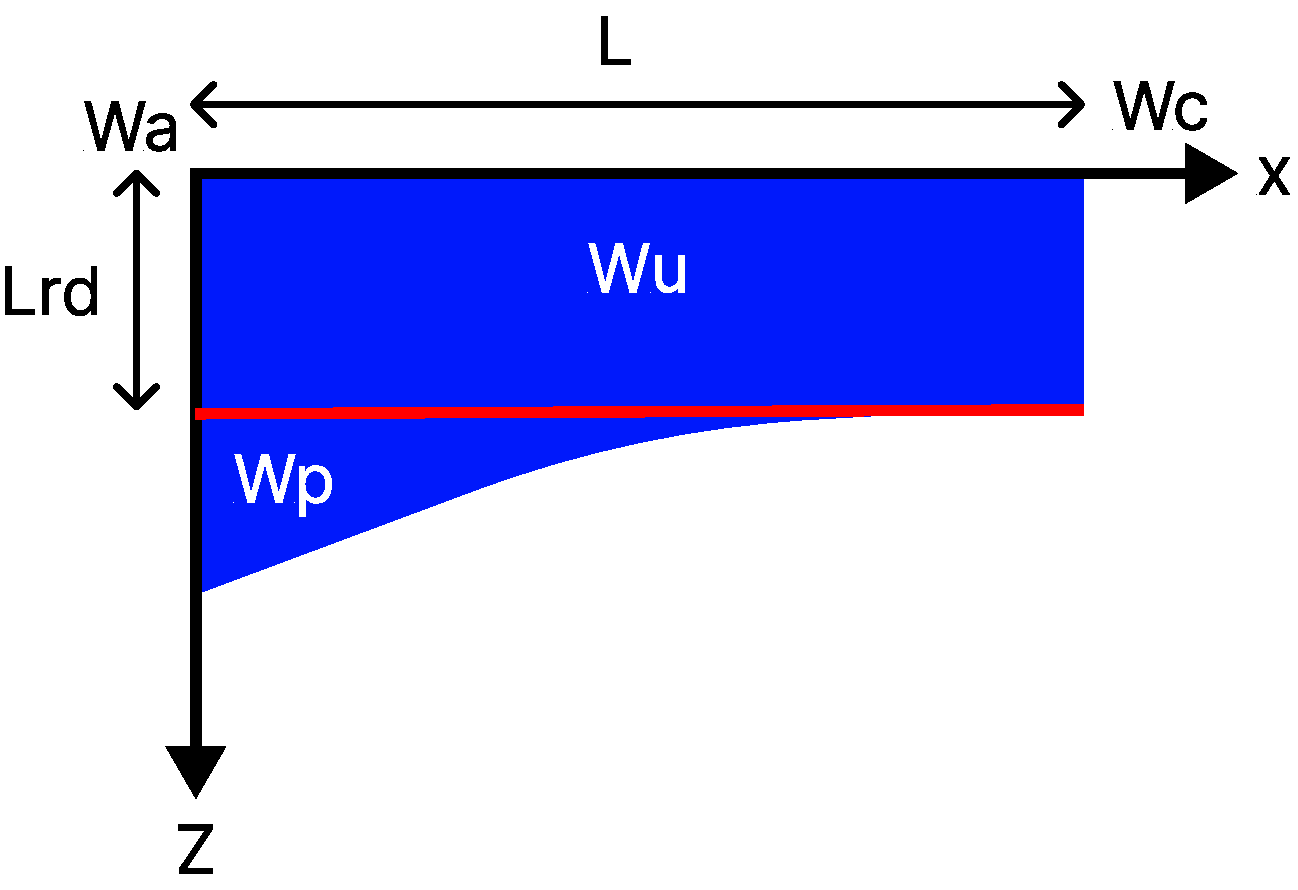
\includegraphics[width=0.5\textwidth]{r22.pdf}
  \caption{Diagrama de distribución de agua en el riego por gravedad}
  \label{r22}
\end{figure}
\begin{equation}
    W_a = W_u + W_p+ W_c
\end{equation}
\begin{notation}
    \begin{itemize}
        \item $W_a$ Agua aplicada (entregada en la cabecera de la melga $L^3$)
        \item $W_u$ Agua útil $L^3$
        \item $W_p$ Agua percolada $L^3$
        \item $W_c$ Agua de coleos $L^3$
    \end{itemize}
\end{notation}
\subsubsection{Eficiencia de aplicación}
La eficiencia de aplicación del riego es el cociente entre la cantidad de agua que queda disponible en la zona de raíces de los cultivos (útil, con fines de evapotranspiración para los cultivos), y la cantidad de agua aplicada al campo irrigado, esto es :
\begin{equation}
    E_a = \frac{W_u}{W_a} \cdot 100
\end{equation}
\begin{notation}
    \begin{itemize}
        \item $E_a$ eficiencia de aplicación del riego \%
        \item $W_u$ cantidad de agua útil [$L^3$ o $L^3/L^2$]
        \item $W_a$ cantidad de agua aplicada [$L^3$ o $L^3/L^2$]
    \end{itemize}
\end{notation}
La diferencia $(100-E_a)$m representa el porcentaje de agua que se desperdicia, que en el riego por gravedad ocurre principalmente debido a percolación profunda y/o escurrimiento superficial (coleos).

La eficiencia de aplicación del requerimiento se define como el cociente entre la cantidad de agua útil t la cantidad de agua que se desea o se requiere incorporar en la zona de raíces de los cultivos:
\begin{equation}
    E_{ar}= \left(\frac{W_u}{W_r}\right) \cdot  100
\end{equation}
\begin{notation}
    \begin{itemize}
        \item $E_{ar}=$ Eficiencia de aplicación del requerimiento
        \item $Wu =$ Cantidad de agua útil, [$L^3 o L^3/L^2$]
        \item $Wr =$ Cantidad de agua requerida, [$L^3 o L^3/L^2$]
    \end{itemize}
\end{notation}
La diferencia (100 -$ E{ar}$), representa el porcentaje de agua que se dejó de apl

En el riego por gravedad, no puede existir una Eficiencia de riego no puede ser mayor al 100\%

\subsubsection{Coeficiente de uniformidad de Christiansen}
Se calcula con la siguiente expresión:
\begin{equation}
    CU_c = \left(\frac{\sum_{i = 1}^{N} \left\lvert Z_i - \bar{Z} \right\rvert  }{N\bar{Z}}\right) \cdot 100
\end{equation}
\begin{notation}
    \begin{itemize}
        \item $CU_c$= Coeficiente de uniformidad de Christiansen \%
        \item $Z_i$= Lámina de agua infiltrada en el i-esimo punto a lo largo de la melga o surco
    \end{itemize}
\end{notation}
El coeficiente de uniformidad de Christiansen con los datos de láminas infiltradas, conduce a un valor de $CU_c= 96.6\%$ aclarando que en el proceso de cálculo se utilizaron sólo cinco láminas (el promedio entre cada par consecutivo de las reportadas en el cuadro) para utilizar láminas con el mismo grado de representatividad
\begin{table}[h!]
    \centering
    \begin{tabular}{@{}cccc@{}}
    \toprule
    \multirow{2}{*}{Parámetro} &
      \multicolumn{3}{c}{\begin{tabular}[c]{@{}c@{}}Clasificación del riego\\ resultante\end{tabular}} \\ \cmidrule(l){2-4} 
     &
      \begin{tabular}[c]{@{}c@{}}Riego\\ malo\end{tabular} &
      \begin{tabular}[c]{@{}c@{}}Riego\\ satisfactorio\end{tabular} &
      \begin{tabular}[c]{@{}c@{}}Riego\\ bueno\end{tabular} \\ \midrule
    Eficiencia de aplicación \% &
      \textless{}60 &
      60-75 &
      \textgreater{}75 \\
    \begin{tabular}[c]{@{}c@{}}Eficiencia de aplicación\\ del requerimiento \%\end{tabular} &
      \textless{}80 &
      80-90 &
      \textgreater{}90 \\
    \begin{tabular}[c]{@{}c@{}}Coef. de uniformidad de\\ Christiansen \%\end{tabular} &
      \textless{}80 &
      80-90 &
      \textgreater{}90 \\ \bottomrule
    \end{tabular}
    \caption{Calidad de riego resultante en base sus parámetros de eficiencia y uniformidad}
    \label{tabr7}
\end{table}
\begin{example}
    En una evaluación de riego por melgas, con el extremo final abierto, se obtubieron los siguientes datos:
    \begin{itemize}
        \item Longitud de melga: 150 m
        \item Ancho de melga: 12 m
        \item Caudal: 32 lps
        \item Tiempo de riego: 125 min
        \item Función de Infiltración $z= 1.561\cdot t^{0.39}$ (cm,min)
        \item Lámina de riego por aplicar: 10 cm
    \end{itemize}
    \begin{table}[h!]
        \centering
        \begin{tabular}{@{}c|cccccc@{}}
        \toprule
        Distancia, m  & 0   & 30  & 60  & 90  & 120 & 150 \\
        Avance, min   & 0   & 6   & 15  & 28  & 47  & 72  \\
        Recesión, min & 125 & 127 & 130 & 135 & 145 & 160 \\ \bottomrule
        \end{tabular}
        \caption{Datos del avance y la recesión}
        \label{tabrg}
    \end{table}
    \textit{ Sol. }

Una representación gráfica del proceso del avance y recesión se muestra en la figura \ref{r}, en la forma acostumbrada para hacerlo, es decir, ubicando en el ejen horizontal las distancias desde la cabecera de la melga (cadenamientos) y en el eje vertical el  tiempo transcurrido. En esta figura también  se expresa gráficamente el concepto de  tiempo de oportunidad. Nótese que se  esperará mejor uniformidad en el riego, a  medida que las curvas de avance y recesión  sean ``más paralelas''
\begin{figure}[h!]
    \centering
      \includegraphics[width=0.5\textwidth]{r26.pdf}
      \caption{Curva de avance y recesión del ejemplo de evaluación}
      \label{r26}
    \end{figure}
\begin{table}[h!]
    \centering
    \begin{tabular}{@{}ccccc@{}}
    \toprule
    \begin{tabular}[c]{@{}c@{}}(1)\\ Distancia,\\ m\end{tabular} &
      \begin{tabular}[c]{@{}c@{}}(2)\\ Tiempo de\\ Avance, min\end{tabular} &
      \begin{tabular}[c]{@{}c@{}}(3)\\ Tiempo de\\ Recesión, min\end{tabular} &
      \begin{tabular}[c]{@{}c@{}}(4)\\ Tiempo de\\ Oportunidad,\\ min\end{tabular} &
      \begin{tabular}[c]{@{}c@{}}(5)\\ Lámina\\ Infiltrada, cm\end{tabular} \\ \midrule
    0   & 0  & 125 & 125 & 10.3 \\
    30  & 6  & 127 & 121 & 10.2 \\
    60  & 15 & 130 & 115 & 10.0 \\
    90  & 28 & 135 & 107 & 9.7  \\
    120 & 47 & 145 & 98  & 9.4  \\
    150 & 72 & 160 & 88  & 9.0  \\ \bottomrule
    \end{tabular}
    \caption{Cálculo de la lámina infiltrada del ejemplo de evaluación}
    \label{tabr8}
    \end{table}
\begin{example}
En el cuadro \ref{tabr8} se muestra el proceso de cálculo de las láminas infiltradas en cada punto donde se tomó el tiempo de avance y recesión (cada 30 m). Las columnas (1), (2) y (3) son los datos de campo; la columna (4) corresponde al tiempo de oportunidad, es decir la diferencia entre el tiempo de recesión y el tiempo de avance (columna 3 menos columna 2); la columna (5) tiene los valores de láminas infiltradas, calculadas sustituyendo el tiempo de oportunidad en la función de infiltración acumulada.

Las láminas infiltradas pueden representarse gráficamente, para obtener el patrón de láminas infiltradas (figura 2). Esta gráfica es bastante descriptiva de lo ocurrido durante el proceso de riego: puede observarse el área que no se regó suficientemente (al final de la melga), así como aquella porción de la melga donde ocurrieron pérdidas por percolación profunda.
% \begin{figure}[h!]
%     \centering
%       \includegraphics[width=0.5\textwidth]{r27.pdf}
%       \caption{Patrón de láminas infiltradas del ejemplo de evaluación}
%       \label{r27}
% \end{figure}
A partir de los datos del cuadro 1 y teniendo presente lo que se observa en la figura \ref{r27}, se puede comprender que la cantidad total de agua que se entregó en la cabecera de la melga, quedó distribuida de la siguiente manera: una parte quedó dentro de la zona de raíces de los cultivos y por lo tanto es la parte que será utilizada por la planta en el proceso evapotranspirativo, la cual llamaremos agua útil; otra parte del agua entregada, se infiltró más allá de la zona radicular de los cultivos, la cual llamaremos pérdidas por percolación profunda; finalmente, otra parte salió por el extremo final de la melga y la llamaremos pérdidas por escurrimiento superficial o pérdidas por coleo.
\end{example}
La cantidad de agua aplicada en la cabecera de la melga ($W_a$), puede calcularse mediante el producto del caudal aplicado y el tiempo de riego para nuestro ejemplo es:
\begin{equation*}
    W_a = 0.032 (125 \cdot 60) = 240 m^3
\end{equation*}
El agua útil y las pérdidas por percolación

Las pérdidas por coleo se pueden estimar por diferencia, es decir despejando esta incógnita (suponiendo que no fuer medido en campo)
\begin{equation*}
    W_c = 240 - 174.96 - 1.26 =
\end{equation*}
También es conveniente conocer la cantidad de agua requerida, la cual denominaremos $W_r$ y puede calcularse mediante:
\begin{equation}
    W_r = L_{rn} \cdot L \cdot A
\end{equation}
\begin{notation}
    \begin{itemize}
        \item $W_r$ Cantidad de agua requerida en $m^3$ (aunque)
    \end{itemize}
\end{notation}

Para el caso del ejemplo, la eficiencia de aplicación resulta:
\begin{equation}
    E_a = \left(\frac{74.96}{240}\right) \cdot 100 = 72.9\%
\end{equation}

De acuerdo con el cuadro, el riego evaluado es satisfactorio por su eficiencia de aplicación y riego bueno por su eficiencia de aplicación del requerimiento y su coeficiente de uniformidad.

Resulta además de gran utilidad expresar las pérdidas por percolación profunda y por coleo en forma porcentual con respecto al agua total aplicada a la parcela. De esta manera, y teniendo presente los valores de los tres parámetros analizados, se tendrán mejores elementos para sugerir medidas para mejorar el riego evaluado. 

Las pérdidas porcentuales por percolación profunda son:
\begin{equation*}
    PP = \left(\frac{1.26}{240}\right) \cdot 100 = 0.5\%
\end{equation*}
Las pérdidas porcentuales por coleo son:
\begin{equation*}
    PC = \left(\frac{63.78}{240}\right) \cdot 100 = 26.6\%
\end{equation*}
Esto significa que las pérdidas porcentuales totales (percolación + coleo) son de 27.1\%, lo cual está de acuerdo con el valor de eficiencia de aplicación obtenido anteriormente (72.9\%)
\end{example}
Más aún, esto permite sugerir algunas medidas para mejorar el riego evaluado. Para nuestro ejemplo, y tomando en cuenta que los coleos son las pérdidas más importantes, se puede sugerir cerrar el extremo final de la melga, con la idea de abastecer el déficit al final de la parcela; aunque quizás más importante sería disminuir un poco el caudal de riego y/o el tiempo de riego, con lo que se logrará una mejora de la eficiencia de aplicación.
\subsection{Enfoques de Diseño del Riego por Gravedad}
El objetivo es revisar los enfoques de diseño del Riego por Gravedad, de acuerdo a
\begin{itemize}
    \item El tipo de diseño requerido;
    \item La disponibilidad de información; y
    \item El contexto de su evolución histórica
\end{itemize}
\subsubsection{Tipos de diseño} 
Los enfoques de diseño y análisis pueden variar
dependiendo si se trata de:
Un diseño preliminar (etapa de
planeación y construcción de la
infraestructura);
\begin{itemize}
    \item Un diseño detallado;
    \item Un diseño libre; o,
    \item Un diseño condicionado
\end{itemize}
\subsubsection{Información disponible}
La diversidad de enfoques de diseño y análisis
del riego por gravedad se explica por:
\begin{itemize}
    \item La mayor o menor información disponible;
    \item La existencia o no de infraestructura de riego, así como la disponibilidad de agua (posibilidad de realizar pruebas de riego); y,
    \item La existencia o no de una sistematización de los predios en campo (incluyendo la posibilidad de que ya se tengan construidas las melgas o surcos)    
\end{itemize}
\subsubsection{Diseño}
En un sentido amplio (diseño completo), el problema
de diseño del riego por gravedad (melgas o surcos),
consiste en:
\begin{enumerate}
    \item Elegir la dirección de riego, lo cual implica definir o adoptar una pendiente en el sentido del riego
    \item Determinar la geometría de las melgas o surcos
    \item Definir el caudal a aplicar
    \item Definir el tiempo de riego (tiempo de aplicación).
\end{enumerate}
Para efectuar un diseño completo, se requieren conocer los datos siguientes:
\begin{enumerate}
    \item Lámina de riego de diseño
    \item Tipo de suelo (Textura e infiltración). Función de infiltración acumulada e infiltración básica
    \item Plano del predio (geometría y pendientes generales)
    \item Caudal disponible en regadera
    \item Caudal máximo no erosivo
\end{enumerate}
Las variables involucradas y responsables del resultado final del riego (caracterizado por las eficiencias obtenidas) son:
\begin{enumerate}
    \item Lámina de riego por aplicar
    \item Longitud y ancho de melga o surco
    \item Tipo de suelo (características de infiltración)
    \item Pendiente en el sentido del riego
    \item Caudal
    \item Tiempo de aplicación
    \item Resistencia al flujo
\end{enumerate}
Las variables se pueden catalogar como:
\begin{itemize}
    \item Parámetros de diseño (datos) \begin{itemize}
        \item Lámina de riego
        \item Infiltración
        \item Pendiente
        \item Longitud de melga o surco
        \item Rugosidad (resistencia al flujo)
    \end{itemize}
    \item Variables de diseño (variables de estado o resultados) \begin{itemize}
        \item Ancho (dentro de ciertos límites prácticos)
        \item Caudal
        \item Tiempo de riego
    \end{itemize}
\end{itemize}
Maximizar la eficiencia de aplicación, con:
\begin{itemize}
    \item Ear = 100\% ó $\leq 90$\%;
    \item Cuc $\leq 90$\%; y,
    \item sin riesgo de erosionar al suelo.
\end{itemize}
Los enfoques de diseño son:
\begin{enumerate}
    \item Tablas y/o gráficas de diseño (Guía general o diseño preliminar)
    \item Pruebas de campo: caudal máximo no erosivo, avance, infiltración
    \item Métodos empíricos, quasi-analíticos o soluciones simplificadas
    \item Modelos matemáticos de mayor o menor grado de simplificación (desde los modelos hidrológicos o de balance de volumen, hasta los modelos hidrodinámicos completos)
\end{enumerate}
\section{Hidráulica del riego por gravedad}
Presentar las bases teóricas del movimiento del agua en el riego por gravedad

En el riego por gravedad ocurren en forma simultánea dos tipos de flujo:
\begin{itemize}
    \item Un flujo superficial
    \item Un flujo subterráneo (infiltración)
\end{itemize}
Ambos escurrimientos son de tal complejidad, que dificultan su tratamiento matemático riguroso

\begin{definition}[Flujo superficial]
    El tipo de flujo superficial que ocurre durante
el riego por gravedad es:
\begin{itemize}
    \item Variable (sus características hidráulicas varían en el espacio)
    \item Transitorio (sus características hidráulicas varían en el tiempo)
\end{itemize}
Para fines prácticos se considera que el
movimiento que se da sobre la superficie
del suelo es unidimensional.
\end{definition}


\begin{definition}[Flujo superficial]
    Este movimiento es esencialmente vertical y prácticamente ocurre en condiciones de no saturación.
\end{definition}

Otras dificultades para el estudio analítico del riego por gravedad
\begin{itemize}
    \item Los escurrimientos superficial y subterráneo, además de simultáneos son interdependientes
    \item Existe variabilidad espacial y temporal de algunos parámetros del suelo, tales como la rugosidad y otras características hidrodinámicas
\end{itemize}
Aunque se sabe que:
\begin{enumerate}
    \item El escurrimiento superficial es modelado por las ecuaciones de Saint Venant, que son ecuaciones diferenciales parciales, no lineales y que no tienen solución analítica conocida
    \item El escurrimiento subterráneo es modelado por alguna de las formas de las ecuaciones de conservación de la masa y de la ecuación de Darcy para flujo no saturado (por ejemplo: La ecuación de Richards)
\end{enumerate}
Se revisarán los aspectos hidráulicos de los modelos más sencillos y simplificados

\subsection{Modelos del escurrimiento superficial}
Estos son los modelos de ajuste estadístico, por ejemplo el modelo potencial es:
\begin{equation}
    x = pt^r
\end{equation}
\begin{notation}
    \begin{itemize}
        \item $x=$ distancia
        \item $p=$ 
        \item $t=$ tiempo
        \item $r=$ 
    \end{itemize}
\end{notation}
Uso de la ecuación de Manning $V= \frac{1}{n}r^{2/3}S^{1/2}$ para relacionar las variables de flujo en la cabecera de la melga (flujo somero) o surco.
\begin{table}[h!]
    \centering
    \begin{tabular}{@{}cc@{}}
    \toprule
    $x,m$ & t,min \\ \midrule
    0     & 0     \\
    20    & 5     \\
    40    & 12    \\
    60    & 22    \\
    80    & 35    \\
    100   & 50    \\
    120   & 68    \\
    140   & 88    \\
    160   & 110   \\ \bottomrule
    \end{tabular}
    \caption{Modelos descriptivos del escurrimiento superficial (fase de avance)}
    \label{tabr}
\end{table}
Cuando $d<b$:
\begin{align*}
    &Q=AV = \frac{A}{n} r^{2 /3}S^{1 /2}\\
    &A= bd\\
    &P = b + 2d\\
    &r = \frac{A}{P} = \frac{bd}{b+ 2d}\approx \frac{bd}{b} = d
\end{align*}
Para flujo somero $r\approx d$, considerando ancho unitario b=1, entonces A=bd=d y por lo tanto si $q=Q/b$:
\begin{equation}
    q = AV = \frac{1}{n}d^{\frac{5}{3}}S^{\frac{1}{2}}
\end{equation} 
Estos son los modelos de ajuste estadístico, el modelo de Kostiakov:
\begin{equation}
    Z = kt^a
\end{equation}
\begin{notation}
    \begin{itemize}
        \item $Z=$ infiltración acumulada [L]
        \item $t=$ Tiempo transcurrido [T]
        \item $k,a=$ parámetros de ajuste estadístico [Adim]
    \end{itemize}
\end{notation}
Esta expresión no representa la infiltración en tiempos largos.


Estos son los modelos de ajuste estadístico: Modelo de Kostiakov-Lewis:
\begin{equation}
    Z =kt^a + f_0t
\end{equation}
\begin{notation}
    \begin{itemize}
        \item $Z=$ infiltración acumulada [L]
        \item $t=$ Tiempo transcurrido [T]
        \item $k,a=$ parámetros de ajuste estadístico [Adim]
        \item $f_0=$ infiltración básica [L/T]
    \end{itemize}
\end{notation}

\subsubsection{Modelos predictivos del escurrimiento}
Estos son los modelos físicamente fundamentados, tal como el modelos Green y Ampt (1911):
\begin{equation}
    Z= K_s \cdot t +\lambda \cdot \ln{\left(1 + \frac{Z}{\lambda} \right)}
\end{equation}
\begin{notation}
    Donde $\lambda= \left(h+h_f\right)\left(\theta_s-\theta_0\right)$
    \begin{itemize}
        \item $Z=$ infiltración acumulada [L]
        \item $t=$ Tiempo transcurrido [T]
        \item $K_s$ Conductividad hidráulica a saturación [L/T]
        \item $h=$ Tirante sobre la superficie del suelo [L]
        \item $h_f=$ Presión en el frente de humedecimiento [L]
        \item $\theta_0=$ Contenido de humedad volumétrico inicial del suelo [Adim]
        \item $\theta_s$ contenido de humedad volumétrico a saturación [Adim]
    \end{itemize}
\end{notation}
Para determinar la infiltración:
\begin{itemize}
    \item Cilindros infiltrómetros
    \item Entradas y salidas
    \item Balance de volumen (dos puntos de la trayectoria de avance)
\end{itemize}
\subsubsection{Método de entradas y salidas}
Se afora a la entrada y salida del surco, a al entrada con sifones o con un vertedor y a la salida con un aforador Parshall
\begin{figure}[h!]
\centering
  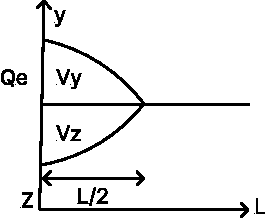
\includegraphics[width=0.5\textwidth]{r23.pdf}
  \caption{Método de los dos puntos}
  \label{r23}
\end{figure}
\begin{equation}
    Q_e \cdot t_{\frac{L}{2}} = V_e = V_y + V_z
\end{equation}
\subsection{Ecuación de momentum}
La aplicación de la segunda ley de Newton al flujo transitorio, que ocurre en el riego por gravedad produce la siguiente ecuación:
\begin{equation}
    \frac{1}{Ag}\cdot \frac{\partial Q}{\partial t} + \frac{2Q}{A^2g} \cdot parti\frac{\partial Q}{\partial x} +\left(1 - Fr^2 \right)\frac{\partial y}{\partial x} = S_0 - S_f
\end{equation}
\begin{notation}
    \begin{itemize}
        \item $A=$ Área de la sección transversal de flujo [$L^2$]
        \item $Q=$ Caudal [$L^3/T$]
        \item $Fr=$ Número de Froude
        \item $W=$ Ancho del espejo del agua [L]
        \item $y=$ Tirante de flujo [L]
        \item $g=$ Aceleración de la gravedad $[L/T^2]$
        \item $t=$ Tiempo [T]
        \item $x=$ Distancia en la dirección de flujo [L]
        \item $S_0=$ Pendiente de la melga o surco [L/L]
        \item $S_f=$ Pendiente de la línea de energía [L/L]
    \end{itemize}
\end{notation}
Esta ecuación, representa el movimiento del agua en suelos parcialmente saturados, y fuer formulada por Lorenzo A. Richards en 1931. Es una ecuación diferencial parcial, no lineal, la cual es difícil de aproximar, puesto que no tiene solución analítica.

La ley de Darcy fue desarrollada para flujo en medios porosos saturados. A ésta Richards le aplicó un requisito de continuidad, sugerido por Buckingham y obtuvo una ecuación general diferencial parcial que describe el movimiento del agua en suelos no saturados que no se expanden. Desde entonces, esta ecuación es conocida como la Ecuación de Richards:
\begin{equation}
    \frac{\partial \theta}{\partial t} = \frac{\partial }{\partial Z} \left[ K(\theta) \left(\frac{\partial \psi }{\partial z} + 1 \right) \right] 
\end{equation}
\begin{notation}
    \begin{itemize}
        \item $K=$ Conductividad hidráulica
        \item $\psi=$ Carga de presión
        \item $Z=$ Elevación con respecto un nivel de referencia
        \item $\theta$ Es el contenido de humedad volumétrico y 
        \item $t=$ Tiempo
    \end{itemize}
\end{notation}
\section{Diseño de melgas con pendiente}
\subsection{Gráficas de Diseño}
Ancho máximo de melga
\begin{equation}
    A = \frac{5}{S}
\end{equation}
Gráfica Pendiente Transversal en \% (S) - Ancho de la melga en m (A)
\begin{align*}
    S(\%) = \frac{\Delta Z}{DH} \cdot 100 &&a &&a
\end{align*}

Longitud máxima de melga, Gráfica Infiltración básica (cm/h) - Longitud de tirada (m)


Caudal por metro de ancho de melga, gráfica de Infiltración básica (cm/h) - Caudal por metro de ancho de melga (L/S/m)
% TODO
\begin{align*}
    DH= \frac{\Delta z}{S(\%)}\cdot 100&& DH= A=\frac{a}{a}
\end{align*}

\begin{example}
    Se tiene un terreno, bien nivelado y casi cuadrado, de 312m por 303m, con la mayor pendiente sobre el laod corto, del ordend de 0.5\% y una pendiente transversal de 0.4\%.

    En el terreno se pretende establecer alfalfa para regarse por melgas, las cuales deberán diseñarse para lograr la mayor eficiencia de aplicación. El terreno es de textura franca y se estima una infiltración básica de 2cm/hr. Para el riego se dispone de agua de un pozo que descarga un caudal de 32 litros por segundo y de acuerdo con las características del suelo, cultivo y criterio de manejo del riego (como se explicó en el curso de Relación Agua Suelo Planta), se pretende aplicar una lámina de 10cm por riego.
\end{example}

\textit{Sol. }

Tomando en cuenta la pendiente del terreno, el trazo de las melgas podría hacerse para construirlas buscando la mayor pendiente, s decir sobre el lado más corto. En este caso, de acuerdo con la figura, para la pendiente de 0.5\% y una infiltración básica de 2cm/hr 
\begin{figure}[h!]
    \centering
    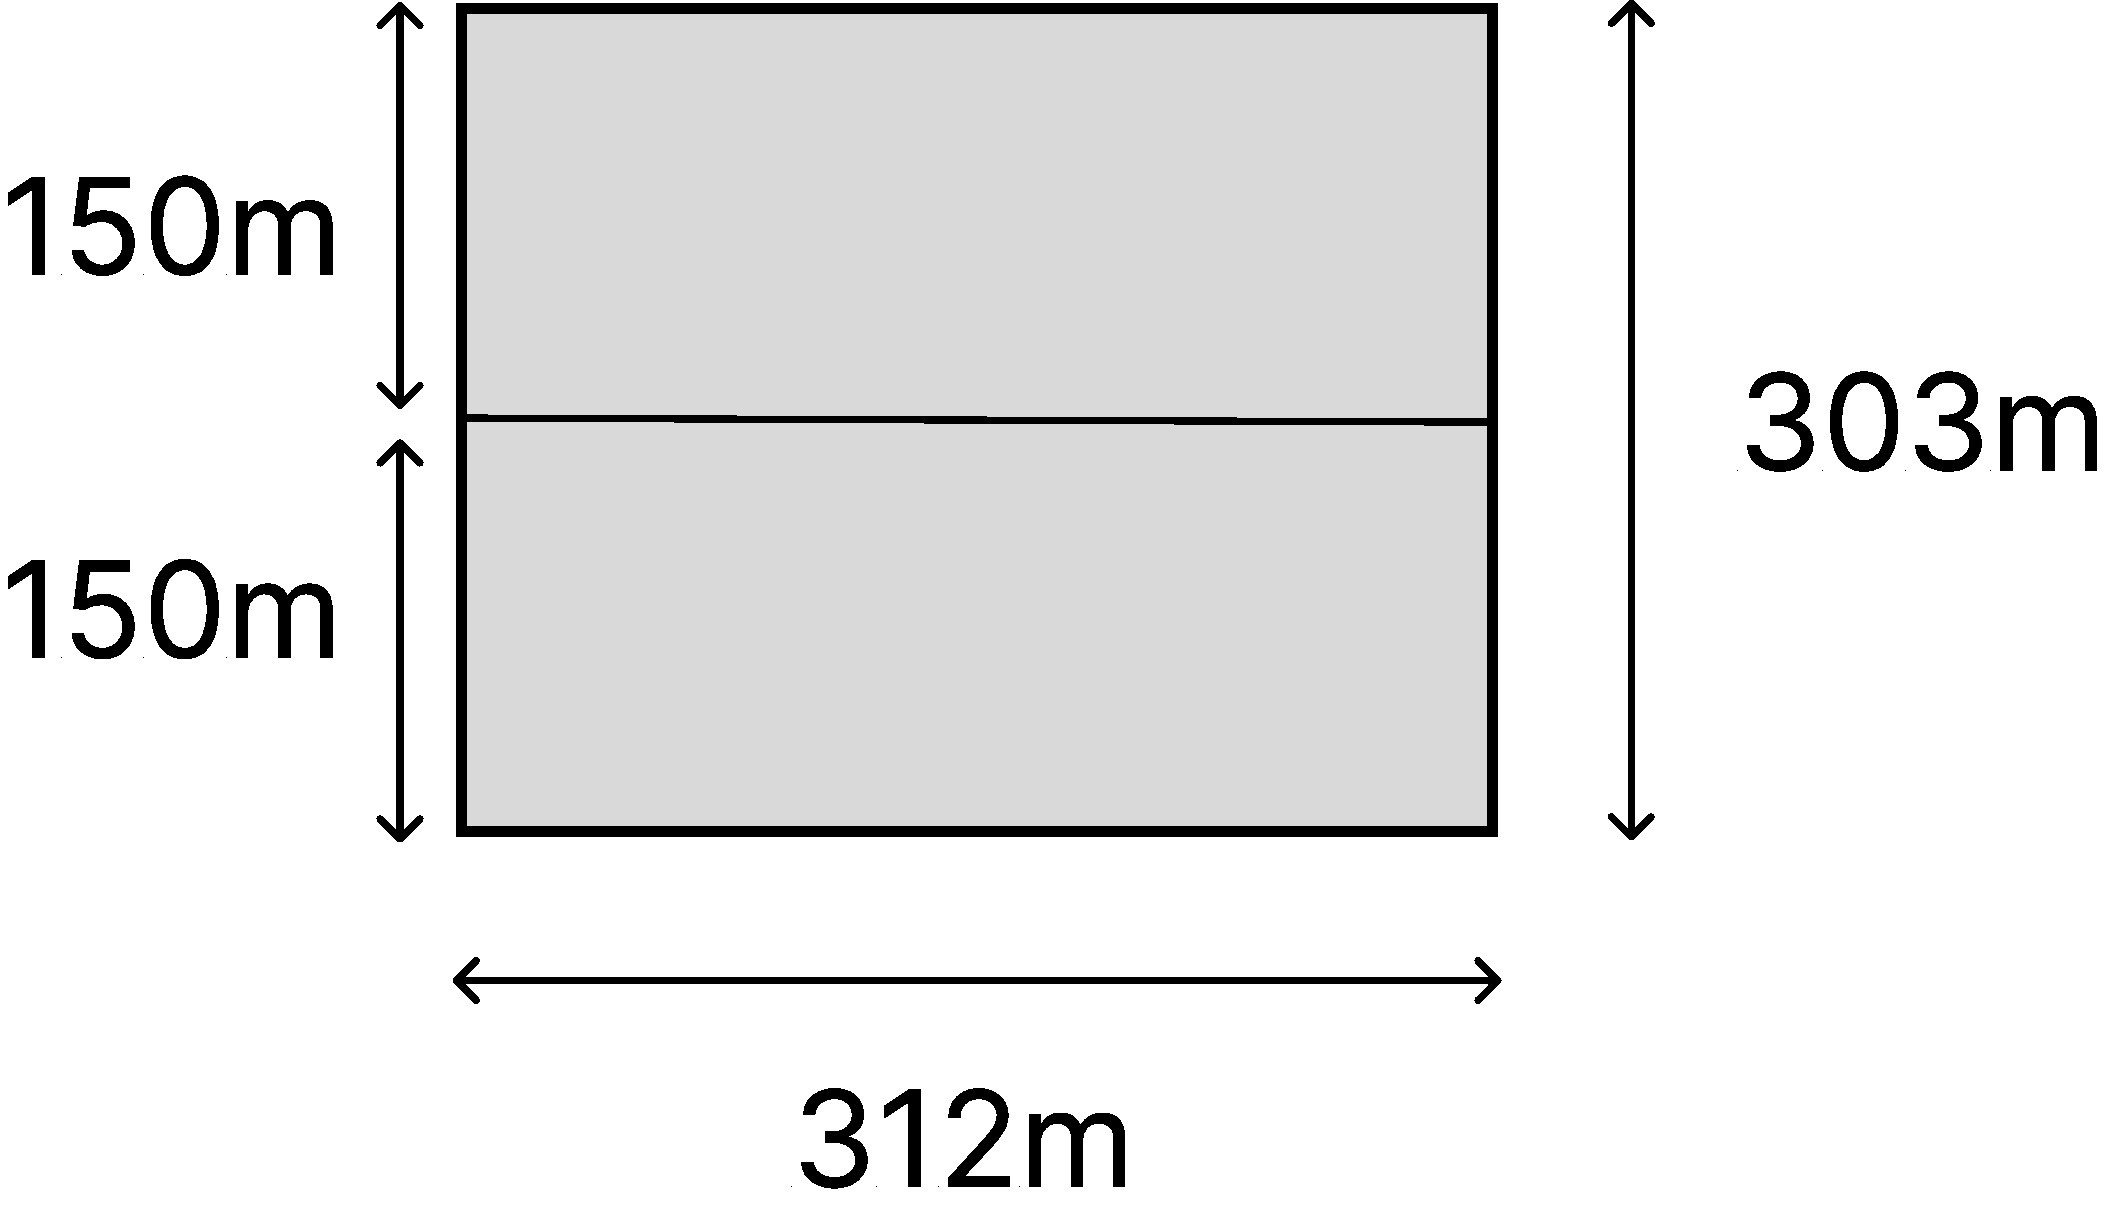
\includegraphics[scale=0.3]{r24.pdf}
    \caption{Cultivo de alfalfa, lb=2cm/hr, el gasto del dispositivo es de 32lps}
    \label{r24}
\end{figure}
El ancho de las melgas se puede obtener en funcipon de la pendiente transversal, considerándose un máximo desnivel de 5cm

De la figura, se obtiene que el ancho podría ser de 21.5m. Sin embargo, es conveniente que quede un número entero de melgas en el ancho

El caudal recomendable se puede obtener de la figura y es de 2.5lps/m; luego, en 12m se requieren 30lps, lo que conduce en forma práctica a utilizar
todo el caudal que descarga el pozo de 32lps

El tiempo de riego recomendable, se calcula con la siguiente ecuación:
\begin{equation}
    Tr=\frac{L\cdot A\cdot Lrd}{6\cdot Q\cdot E_a}
    \label{eqr1}
\end{equation}
\begin{notation}
    \begin{itemize}
        \item $Tr=$ Tiempo de riego en min
        \item $L=$ Longitud de melga m
        \item $A=$ Ancho de melga en m
        \item $Lrd=$ lámina de riego de diseño (neta) cm
        \item $Q=$ Caudal de la melga lps
        \item $Ea=$ Eficiencia de aplicación de proyecto decimal
        \item $6=$ Factor de conversión de unidades
    \end{itemize}
\end{notation}
Suponiendo que se logrará obtener una eficiencia de aplicación de 75\% (eficiencia de diseño), el tiempo de riego será:
    \begin{equation*}
        Tr= \frac{150\cdot 12\cdot 10}{6\cdot 32\cdot 0.75} = 125 min
    \end{equation*}
Los resultados de datos y del diseño son:
\begin{itemize}
    \item Pendiente de riego: 0.5\%, con 2 tablas con 26 melgas cada uno de:
    \item Longitud de melga: 150m
    \item Ancho de melga: 12m
    \item Caudal: 32lps
    \item Tiempo de riego: 125 min
\end{itemize}
\begin{figure}
    \centering
    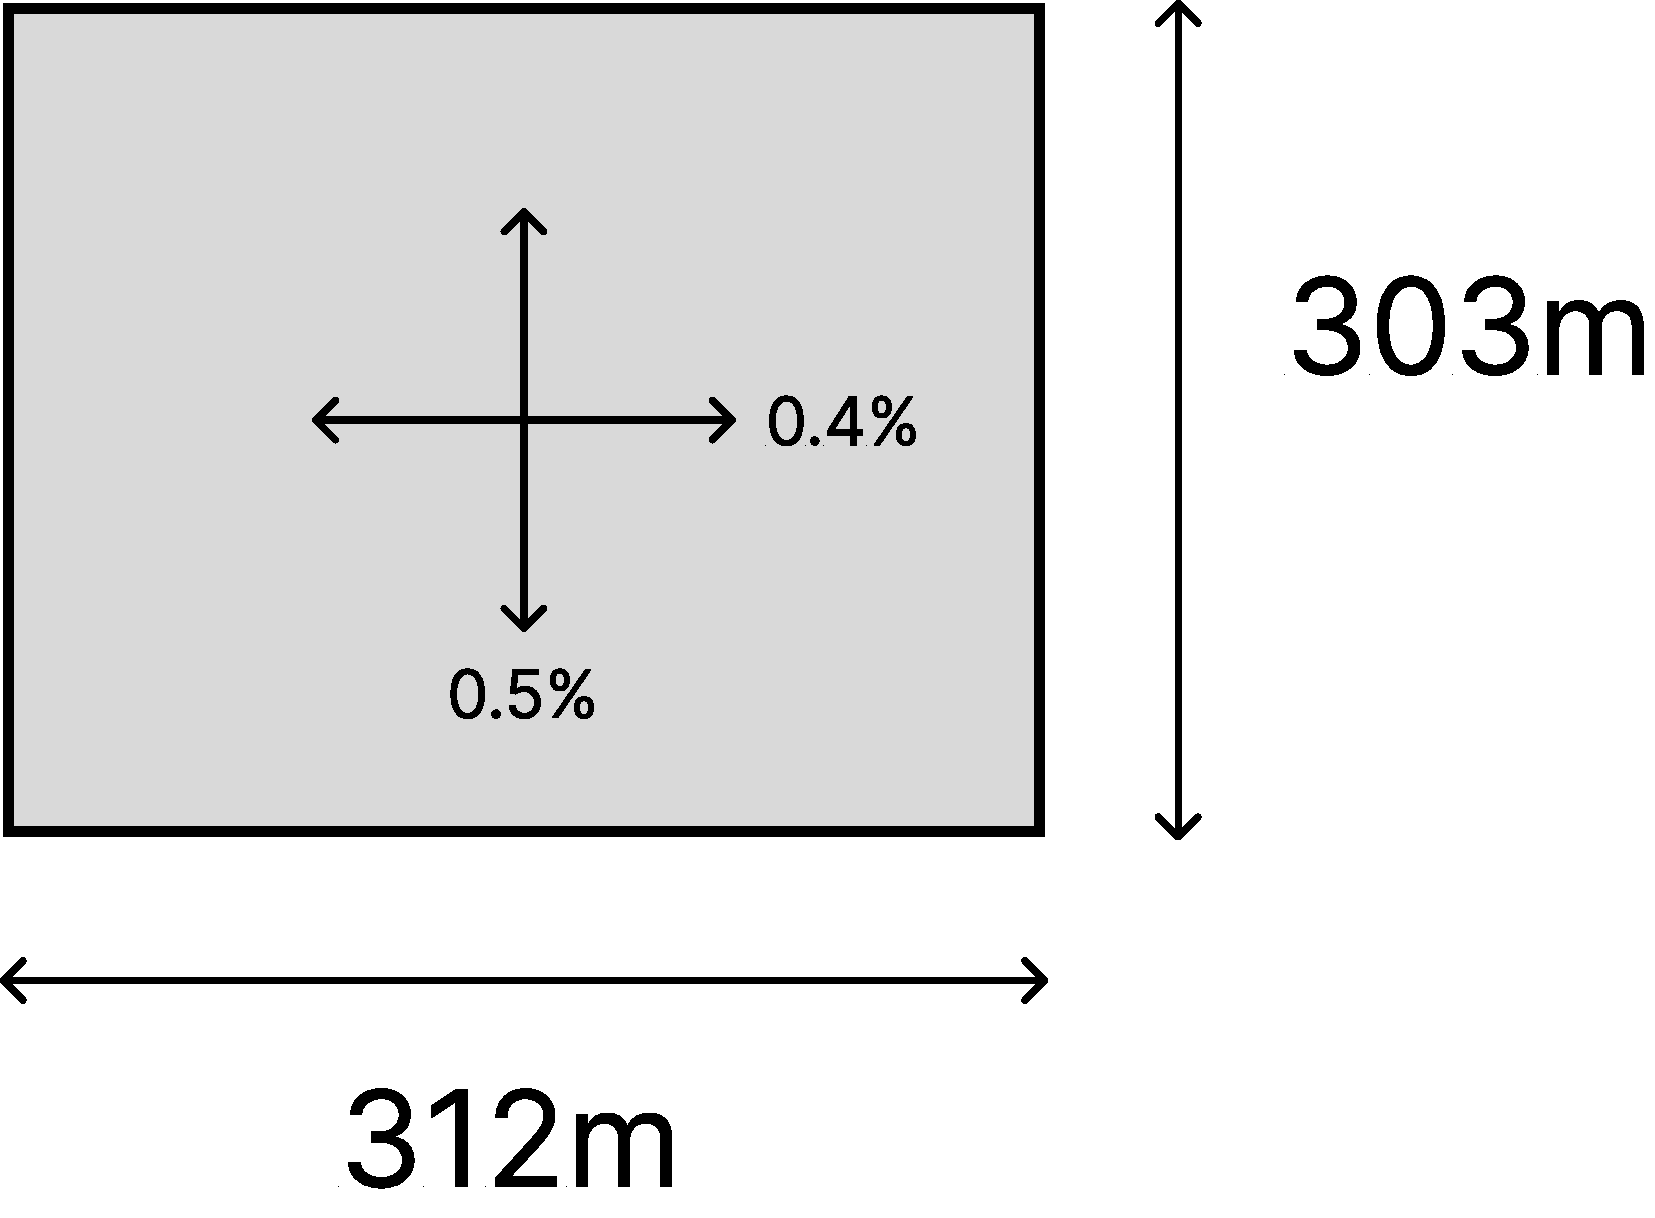
\includegraphics[scale=0.3]{r25.pdf}
    \caption{Del cultivo de alfalfa con lb=2cm/h, Caudal del dispositivo = 32lps (pozo) y Lrd=10cm}
    \label{r25}
\end{figure}

\begin{definition}[Caudal unitario]
    Es el gasto $(q_u)$ necesario para regar eficientemente una superficie de $10m^2$. La magnitud del caudal es directamente proporcional del área de la melga.
\end{definition}
Una vez que se determina el gasto unitario apropiado, para un tipo de suelo, lámina de riego y pendiente dadas, el gasto par cualquier tamaño de melga es simplemente el producto del gasto unitario por el número de áreas unitarias de dicha melga.

Para la determinación del caudal unitario. los autores propusieron originalmente el uso de un nomograma, que relaciona los parámetros de diseño más importantes ($L_{rn}, I_b$ y S), basado en datos de campo de muchos sitios

Los criterios y conceptos complementarios, \textbf{Gasto máximo permisible por erosión}:
\begin{equation}
    q_{\max}= 5.58S^{-0.75}
\end{equation}
\begin{notation}
    \begin{itemize}
        \item $q_{\max}=$ Gasto máximo permisible por erosión L/s/m
        \item S= Pendiente de riego \%
    \end{itemize}
\end{notation}
\textbf{Gasto máximo permisible por tirante:}
\begin{equation}
    q_{\max} = \frac{1000 d^{5/3}S^{1/2}}{n}
\end{equation}
\begin{notation}
    \begin{itemize}
        \item $q_{\max}=$ Gasto máximo permisible por tirante L/s/m
        \item $d=$ Tirante de flujo, m
        \item $n=$ Coeficiente de rugosidad de Manning
        \item $S=$ Pendiente de riego \%
    \end{itemize}
\end{notation}

\textbf{Longitud máxima de la melga:}
Justificación de la fórmula: Del caudal de riego $(Q)$, una vez definido el caudal unitario ($q_u$)
\begin{align*}
    &Q= q_u\frac{LA}{10}\implies q= q_u\frac{L}{10}\\
    &q=q_{\max}\implies q_{\max}= q_u\frac{L_{\max}}{10}
\end{align*}
\begin{equation}
    L_{\max} = \frac{10Q_{\max}}{q_u}
\end{equation}
\begin{notation}
    \begin{itemize}
        \item $q_{\max}=$ Longitud máxima de la melga, m
        \item $q_{\max}=$ Caudal máximo por melga, L/s/m
        \item $q_u=$ Caudal unitario, $L/s/10m^2$
    \end{itemize}
\end{notation}
\textbf{Caudal de riego (q)}:
\begin{equation}
    q= \frac{q_u\cdot L}{10}
\end{equation}

\begin{notation}
    \begin{itemize}
        \item $q_{\max}=$ Caudal de riego L/s/m
        \item $L=$ Longitud de la melga, m
        \item $q_u$ Caudal unitario $L/s/10m^2$
    \end{itemize}
\end{notation}
Y el tiempo de riego, Fórmula \eqref{eqr1}
\section{Diseño y evaluación de melgas}
El problema de aplicar una cantidad de agua de manera eficiente y uniforme a los surcos y melgas, puede resolverse satisfactoriamente, su la dosis de agua proporcionada está de acuerdo con las condiciones locales del terreno (textura, pendiente, estructura, etc)

Estas condiciones locales son difíciles de determinar en forma independiente, por lo que se buscó un método en el que una medida práctica involucrará todos estos factores y su correlación entre ellos.

La hipótesis así planteada, llevó a investigadores en el campo de la Irrigación, a efectuar pruebas de campo en las planicies de Hungría. El resultado de sus investigaciones llevó a una observación práctica que involucrará todos los anteriores factores y que fue precisamente el avance del agua en surcos y melgas en ciertas condiciones que son:

\begin{itemize}
    \item En surcos \begin{itemize}
        \item Gasto: 1 lps/surco
        \item Longitud: 50m
        \item Variable a medir: Tiempo en cubrir los 50m 
    \end{itemize}
    \item En melgas \begin{itemize}
        \item Gasto: 4 lps/m de ancho de melga
        \item Longitud: Primeros 40m y primeros 80m
        \item Variable: Tiempo en cubrir los 40 y 80 m.
    \end{itemize}
\end{itemize}
En base a lo anterior, se llegó a elaborar una serie de tablas de uso práctico, que eliminará las engorrosas evaluaciones de riego en surcos y melgas por los métodos tradicionales, ya que toman mucho tiempo y poco se ajustan a la realidad, puesto que se considera únicamente el criterio y apreciación visual del técnico que efectúa las pruebas

Prueba de campo para surcos:
\begin{enumerate}
    \item Escójase de 5 a 10 surcos que correspondan a las condiciones medias del campo
    \item Tómese una longitud de 50 m
    \item Aplíquese un gasto de 1 lps a cada surco
    \item Tómese el tiempo en que tarda en llegar el frente del agua  a la marca de 50m en cada surco
    \item Obténgase un promedio de los tiempos en que llegaron los frentes de agua a todos los surcos a 50m
\end{enumerate}

La tabla contiene los siguientes datos:
% TABLE
\begin{itemize}
    \item Primer renglón: t= Tiempo utilizado en recorrer el agua 50m con un gasto de 1 lps (minutos)
    \item Segundo renglón: $h\cdot d=$ producto de la lámina por aplicar (mm) y la separación de los surcos (m)
    \item Tercer renglón: T= Tiempo de suministro de agua al surco (minutos) o sea el tiempo de riego
    \item Cuarto renglón primera columna: L= Longitud del surco (m)
\end{itemize}
Todos los datos incluidos por abajo del cuarto renglón y de la segunda columna en adelante, corresponden a los gastos que deberán aplicarse a cada surco (lps)

Los gastos comprendidos entre dos rayas continuas representan una eficiencia de riego del 70 al 80\%

Los gastos incluidos de dos rayas punteadas representan una eficiencia de riego menor del 70\%

Los gastos encerrados en círculo son los gastos óptimos

Los rangos proporcionados en las tablas son:
\begin{itemize}
    \item Lámina por aplicar. De 20 a 200 mm
    \item Longitud de surcos. De 20 a 200m
    \item Producto de la lámina por aplicar por la separación del surco $(hd\cdot d)$: de 20-200 mm-m
    \item Gastos en los surcos: 0.3-3.5 lps
    \item Tiempo de riego: De 15 a 270 minutos
\end{itemize}
\begin{example}
    En un cultivo de Maíz, se tiene una lámina por aplicar de 140mm, y una separación entre surcos: 0.92m

    Los datos de la prueba son: $t_1= 36min, t_1= 36min, t_2= 35 min, t_3= 34 min, t_4= 33 min, t_5= 32 min $
    \textit{ Sol. }

    \begin{align*}
        a
    \end{align*}

    Con los datos obtenidos $\bar{t} = 35min$ y $h\cdot d= 130$, se entra a la tabla correspondiente obteniéndose un tiempo de regado de T= 117 min. y en esa misma columna se encuentran gastos desde 1.7 lps para 90m de longitud, hasta 3.5 lps para una longitud de 190m siendo el gasto óptimo de 2.8 lps.

\end{example}

Primer caso:

Se harán surcos de 150 m de longitud y se dará un tiempo de regado de 117 min con un gasto de 2.8 lps/surco donde se logra la máxima eficiencia de riego.

Ahora bien, en la práctica se pueden tener limitantes de estos dos parámetros (longitud y gasto) o por condiciones de facilidad de manejo

Caso dos:

Suponiendo que en el ejemplo anterior se tuviera un gasto fijo de 30 lps y no haya limitante para longitud de surco, se propondría en vez de utilizar 2.8 lps/surco se utiliza 3 lps/surco de tal manera que se puede dividir el gasto total en 10 surcos.

Entrando a la tabla, con los mismos datos fijos de $\bar{t}= 35min$, $h\cdot d= 130$

Caso tres:

Con este mismo ejemplo y si por condiciones de terreno se tiene una longitud fija de 100m y con los mismos datos se entra a la tabla con una $L= 100m$, se obtiene un gasto de 1.8 lps/surco. Aclarándose que en este caso, el gasto obtenido se aleja del óptimo (2.8lps/surco), por lo que baja la eficiencia de riego.

En todas las alternativas el tiempo de regado (T), es de 117 min debiéndose cortar el agua al cabo de este tiempo, sin importar el hecho de que el agua haya llegado o no a la longitud de surco determinada en cada caso.

Recomendaciones generales:
\begin{itemize}
    \item El sitio seleccionado para la prueba debe representar lo mejor posible las condiciones medias del terreno
    \item En caso de variar estas condiciones, incluyendo el desarrollo del cultivo, se deberán hacer los ajustes efectuando nuevas pruebas
    \item Antes de decidirse
    \item para lograr un resultado satisfactorio, durante la prueba debe garantizarse mantener el gasto constante
    \item Es conveniente efectuar otra prueba cuando el cultivo está en pie, para ajustar el tiempo de riego
\end{itemize}

\section{Riego por descargas intermitentes}
A fines de los 70s, Stringham y Keller (1979), buscando dispositivos para reducir el caudal descubrieron la intermitencia.

A principios de los 80s, se desarrolló una tecnología para crear el riego por descargas intermitentes, bautizándose con el nombre de Surge flow, también denominada pulsed flow (P\&R Surge Systems, 1988)

Es la aplicación del agua en forma intermitente, es decir, mediante una serie de aplicaciones y suspensiones alternadas del caudal de riego (ciclos), hasta completar el tiempo de riego.

Un ciclo completo se compone de dos intervalos de tiempo idénticos; uno durante el cual se aplica el caudal (cycle on-time) y el otro el cual se suspende el suministro (cycle off-time)

Del segundo intervalo de aplicación en adelante, el agua avanzará una distancia progresivamente mayor sobre terreno mojado, haciéndolo con una velocidad mayor que cuando el agua transite sobre terreno seco.

Efectivamente, el mojado previo de los surcos reduce la absorción de agua (velocidad de infiltración) y deja una superficie sellada y lisa que permite una mayor velocidad del agua para alcanzar el final del surco.
% Figura
En la figura, se muestra un esquema típico de infiltración en riego continuo y riego por pulsos en el cual se puede observar que la velocidad de infiltración se reduce al nivel de la infiltración básica, después del primer pulso y se mantiene a ese nivel hasta el final del riego. Cabe aclarar que el logro de este efecto depende del manejo de los tiempos de ciclo.

Comparado con el riego a flujo continuo (caudal constante), el riego por descargas intermitentes alcanzará el final de los surcos, en pozo más del mismo tiempo que lo hará con flujo continuo, pero regando el doble de surcos.

Esto se traduce en un ahorro de alrededor del 25\% de agua cuando se riega por descargas intermitentes, con respecto al riego con caudal continuo (Hernández y Martínez, 1992)

El equipo básico del riego consiste en una tubería de alimentación, que puede ser enterrada o superficial, o bien manguera plana (layflat), la válvula para crear la intermitencia, un controlador electrónico que programa y ejecuta los tiempos de intermitencia, y dos líneas de tuberías con compuertas que se colocan en las cabeceras de los surcos.










































% \subsection{Enfoques de diseño y análisis de los métodos de riego por gravedad}
% \subsection{Hidráulica del riego por gravedad}
% \subsection{Modelos matemáticos en el riego por gravedad}






